\documentclass[11pt]{mk-polish-lab-report}

\usepackage{lipsum}
\usepackage[normalem]{ulem}
%\usepackage[light, math]{anttor}
\usepackage{array,multirow}

\usepackage{latexsym,amsmath,amssymb,amsthm}
\usepackage{multicol}
\renewcommand{\arraystretch}{1,25}
%\usepackage{amssymb}
\usepackage{breqn}
\usepackage{graphicx}

\let\times\relax% Set equal to \relax so that LaTeX thinks it's not defined
\DeclareMathOperator{\times}{\cdot}
\usepackage{subfig}
\graphicspath{ {plots/} }


%\sisetup{ exponent-product=\cdot}

\university{Politechnika Wrocławska}
\major{Informatyka, inż. I st.}
\tutor{dr hab. Paweł Zieliński}
\coursegroup{czwartek TN, 11:15}

\author{Miriam Jańczak}
\studentnumber{229761}
\title{Obliczenia naukowe}
\topic{Lista 2}


%% Uncomment to change margins size
%\geometry{top=2.5cm,bottom=2cm,left=2.5cm,right=2.5cm}

%% Uncomment to change vspace between items in lists
\setlist[enumerate]{itemsep=0pt}
%\setlist[itemize]{itemsep=0pt}
%\setlist[description]{itemsep=0pt}



\begin{document}

\maketitle

\section{Iloczyn skalarny raz jeszcze}

\subsection{Opis problemu}
Ponowne obliczenie iloczynu skalarnego z zadania~5 z listy~1 dla typów \texttt{Float32} i \texttt{Float64} po wprowadzeniu niewielkich zmian danych w wektorze $x$, tj. obcięciu ostatniej cyfry znaczącej współrzędnych $x_4$ i $x_5$ ($9$ dla $x_4$, $7$ dla $x_5$). W tym celu wykorzystano te same cztery algorytmy co w zadaniu z listy~1. Poniżej przedstawiono zmienione dane wejściowe:
\begin{align}
\tilde{x} = &[2.718281828, -3.141592654, 1.414213562, 0.577215664, 0.301029995] \nonumber \\
y = &[1486.2497, 878366.9879, -22.37492, 4773714.647, 0.000185049] \nonumber
\end{align}

\subsection{Rozwiązanie}
Iloczyn skalarny dla typów \texttt{Float32} i \texttt{Float64} obliczono za pomocą czterech algorytmów z programu z listy~1: 
%\begin{multicols}{2}
\begin{enumerate}[(a)]
\item \textit{w przód},
\item \textit{w tył},  
\item \textit{od największego do najmniejszego},
\item \textit{od najmniejszego do największego}.
\end{enumerate}
%\end{multicols}

\subsection{Wyniki}
Zestawienie wyników iloczynów skalarnych $x\cdot y$ (zadanie~5 z listy~1) oraz $\tilde{x}\cdot y$ przedstawia \Cref{table:1}.

\begin{table}[h]
        \centering
        \footnotesize
\begin{tabular}{c
		|S[
        table-number-alignment = right,
		table-figures-integer  = 2,
		table-figures-decimal = 7
		]
		|S[
        table-number-alignment = right,
		table-figures-integer  = 2,
		table-figures-decimal = 7
		]
		|S[
        table-number-alignment = right,
		table-figures-integer  = 2,
		table-figures-decimal = 16,
		table-figures-exponent=3
		]
		|S[
        table-number-alignment = right,
		table-figures-integer  = 2,
		table-figures-decimal = 16,
		table-figures-exponent=3
		]}
%\toprule
& \multicolumn{2}{c|}{\texttt{Float32}} & \multicolumn{2}{c}{\texttt{Float64}} \\ \hline
{Algorytm}& { $x\cdot y$} & { $\tilde{x}\cdot y$} & { $x\cdot y$} & { $\tilde{x}\cdot y$} \\ \hline
(a) &-0.4999443&-0.4999443&1.0251881368296672e-10&-0.004296342739891585 \\ 
(b) &-0.4543457&-0.4543457&-1.5643308870494366e-10&-0.004296342998713953 \\ 
(c) &-0.5&-0.5&0.0&-0.004296342842280865 \\ 
(d) &-0.5&-0.5&0.0&-0.004296342842280865 \\ 
%\bottomrule
\end{tabular}
\caption{Iloczyny skalarne $x\cdot y$ oraz $\tilde{x}\cdot y$ obliczone w arytmetykach \texttt{Float32} i \texttt{Float64} przy użyciu danych algorytmów.}
\label{table:1}
\end{table}	

\subsection{Wnioski}

Przeprowadzając analizę danych z tabeli (\ref{table:1}) można łatwo zauważyć, że w arytmetyce \texttt{Float32} zmiany dokonane w wektorze $x$ nie miały wpływu na wyniki (pozostały one takie same). Jest to spowodowane stosunkowo niewielką precyzją tej arytmetyki, a co za tym idzie pewną niedokładnością w przechowywaniu poszczególnych składowych wektora. Ta niedokładność okazała się tutaj na tyle duża, że usunięcie $9$ z $x_4$ nie zmieniło w żaden sposób zapisu wartości w arytmetyce \texttt{Float32}, a zmiana w $x_5$ zaważyła jedynie na najmniej znaczącym bicie zapisu liczby. Nie należy się zatem dziwić że wyniki nie uległy zmianie, jednak to powinno raczej martwić niż cieszyć, gdyż są one bardzo dalekie od poprawnych. Zgoła odmienna sytuacja miała miejsce w arytmetyce \texttt{Float64}. Tutaj wprowadzenie niewielkich zmian rzutowało bardzo mocno na wyniki obliczeń iloczynu skalarnego. Pierwszą rzeczą jaką można zauważyć jest to, że dane przy operacji obliczania iloczynu skalarnego są bardzo wrażliwe na zmiany. Mogłoby się wydawać że dokonanie modyfikacji rzędu $10^{-9}$ nie wpłynie znacząco na otrzymane wyniki, te jednak bardzo się zmieniły. Z drugiej strony, można zauważyć, że rozbieżności pomiędzy iloczynami skalarnymi uzyskanymi z użyciem poszczególnych algorytmów znacznie się zmniejszyły, a nawet powiedzieć że w granicach pewnego dopuszczalnego błędu są takie same, co pozwala z kolei wnioskować, że wynik iloczynu skalarnego w arytmetyce \texttt{Float64} przy zmienionych danych jest w gruncie rzeczy wynikiem poprawnym. Usunięcie ostatnich cyfr po przecinku z $x_4$ i $x_5$ sprawiło że wektory zostały dokładniej zapisane (zmniejszyła się także ich ortogonalność) i arytmetyka okazała się wystarczająca do obliczenia iloczynu skalarnego. Widać zatem wyraźnie, że precyzja arytmetyki odgrywa kluczową rolę wtedy, kiedy mamy do czynienia ze źle uwarunkowanym zadaniem, tj. wtedy kiedy niewielkie względne zmiany danych powodują duże względne odkształcenia wyników. Do rozwiązywania takich zadań należy zatem używać maksymalnej precyzji.

\section{Nietypowa granica}

\subsection{Opis problemu}

Porównanie wykresów funkcji
\begin{align}
f(x) = e^x \ln(1 + e^{-x})
\label{eq:zad2}
\end{align}
%$f(x) = e^x \ln(1 + e^{-x})$
(narysowanych w co najmniej dwóch programach do wizualizacji) z jej granicą $\mathop {\lim }\limits_{x \to \infty}$, a następnie wyjaśnienie zaistniałego zjawiska.

\subsection{Rozwiązanie}

Wykresy funkcji \eqref{eq:zad2} wykonano za pomocą biblioteki \emph{Plotly} (używając różnych typów zmiennopozycyjnych) w języku \emph{Julia}, a także za pomocą pakietu matematycznego \emph{Wolfram Alpha}. Granicę $\mathop {\lim }\limits_{x \to \infty}$ funkcji \eqref{eq:zad2} wyliczono za pomocą biblioteki \emph{SymPy} w języku \emph{Julia} oraz w sposób analityczny.  

\subsection{Wyniki}
Poniżej przedstawiono (\Cref{fig:zad2-plotly}, \Cref{fig:zad2-wa}) otrzymane wykresy funkcji \eqref{eq:zad2}. 

\begin{figure}[h]
\centering
\subfloat[\texttt{Float16}\label{fig:zad2-fl16}]{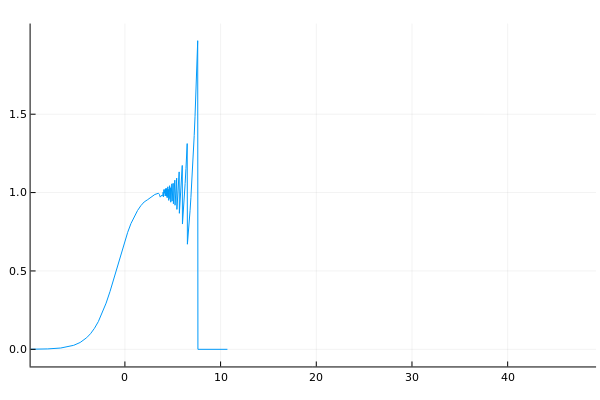
\includegraphics[width=0.5\textwidth]{zad23}}\hfill
\subfloat[\texttt{Float32}\label{fig:zad2-fl32}] {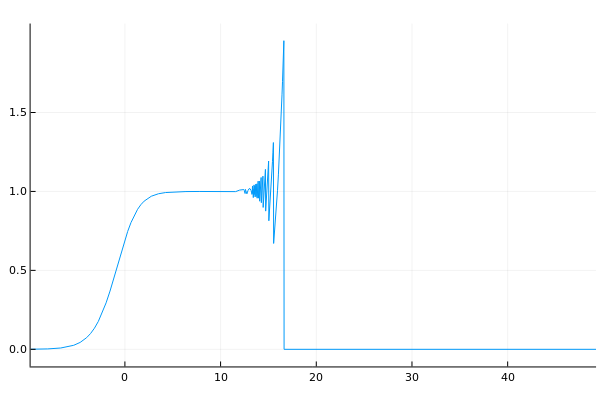
\includegraphics[width=0.5\textwidth]{zad22}}\hfill
\subfloat[\texttt{Float64}\label{fig:zad2-fl64}]{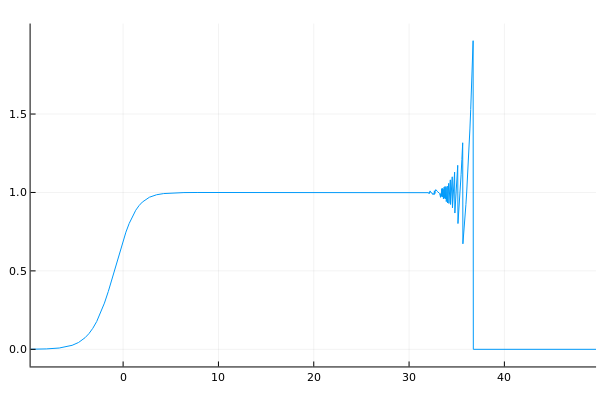
\includegraphics[width=0.5\textwidth]{zad21}}\hfill
\caption{Wykresy wykonane za pomocą biblioteki \emph{Plotly}} \label{fig:zad2-plotly}
\end{figure}

\begin{figure}[h]
\centering
\subfloat[mniejszy zakres \label{fig:zad2-wa1}]{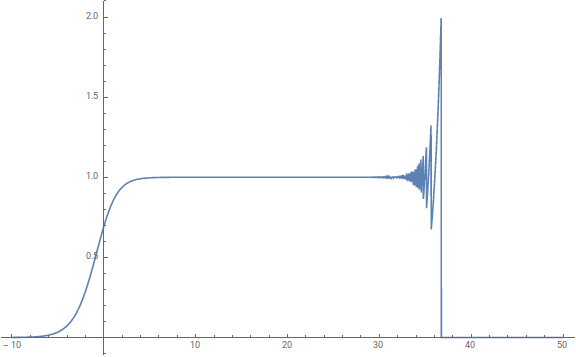
\includegraphics[width=0.49\textwidth]{wa1}}\hfill
\subfloat[większy zakres \label{fig:zad2-wa2}] {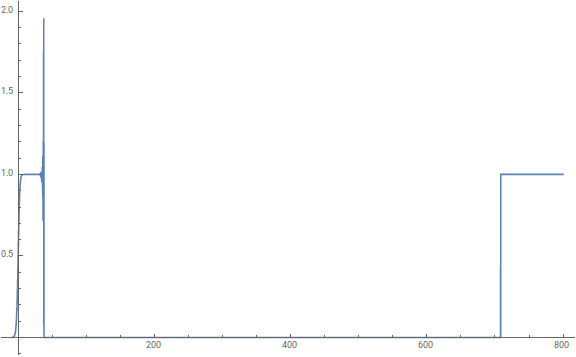
\includegraphics[width=0.49\textwidth]{wa2}}\hfill
\caption{Wykresy wykonane za pomocą programu \emph{Wolfram Alpha}} \label{fig:zad2-wa}
\end{figure}
\noindent Obliczona przez program granica $\mathop {\lim }\limits_{x \to \infty}$ funkcji \eqref{eq:zad2} wynosi $1$. Taki sam wynik został uzyskany przez rozwiązanie analityczne:
\begin{equation}
\begin{aligned}
\mathop {\lim }\limits_{x \to \infty} f(x) &= \mathop {\lim }\limits_{x \to \infty} e^x \ln(1 + e^{-x}) = \mathop {\lim }\limits_{x \to \infty} \dfrac{\ln(1 + e^{-x})}{e^{-x}} = \left[\dfrac{0}{0}\right] \stackrel{H}{=} \mathop {\lim }\limits_{x \to \infty} \dfrac{(\ln(1 + e^{-x}))'}{(e^{-x})'} = \\ 
&= \mathop {\lim }\limits_{x \to \infty} \dfrac{\frac{1}{1 + e^{-x}}\times -e^{-x}}{-e^{-x}} = \mathop {\lim }\limits_{x \to \infty} \dfrac{1}{1 + e^{-x}} = 1. \nonumber
\end{aligned}
\end{equation}

\subsection{Wnioski}

Z analitycznego punktu widzenia oczywistym jest, że dla $x$ dążącego do nieskończoności granica funkcji \eqref{eq:zad2} jest równa jeden. Dużo trudniej natomiast podobnego wyniku dopatrzyć się na wykresach. Na każdym z nich pojawia się bowiem nietypowe zaburzenie, oscylacja niewłaściwa dla funkcji, po której wartości funkcji są równe zero. Na wykresach które przedstawia \Cref{fig:zad2-plotly}, można zaobserwować, że moment pojawienia się owej oscylacji zależny jest od precyzji arytmetyki. Obserwowane zaburzenia wywołane są poprzez dodanie bardzo małej wartości $e^{-x}$ do, w stosunku do niej dużej, jedynki przez co następuje utrata cyfr znaczących. Kluczowe jest jednak pomnożenie logarytmu tak przybliżonej wartości przez bardzo duże $e^{x}$, co potęguje względnie niewielki początkowy błąd i przez co można zaobserwować niepokojące zmiany na wykresie. Łatwo można wnioskować dalej że w momencie kiedy $1 + e^{-x} = 1$ ($e^{-x}$ zostaje całkowicie pochłonięte przez 1), to $\ln(1 + e^{-x}) = 0$, co tłumaczy pojawienie się wartości $0$ na wykresie. W wielu programach wykres funkcji w pewnym momencie się kończy. Wynika to z przepełnienia (\emph{overflow}) dla $e^x$, wtedy pojawia się mnożenie $\infty \times 0$ co przyjmuje wartość \textbf{NaN}. Na wykresie \ref{fig:zad2-wa2} w momencie wystąpienia \emph{overflow} zaobserwować można ,,oszustwo'' jakiego dokonuje program \emph{Wolfram Alpha} podstawiając po prostu wyliczoną analitycznie granicę równą jeden. W tym zadaniu przedstawiona jest sytuacja gdzie małe zmiany danych spowodowały duże odchylenia co pozwala stwierdzić że jest ono źle uwarunkowane.

\section{Układ równań i wskaźnik uwarunkowania}

\subsection{Opis problemu}

Rozwiązanie układu równań liniowych $\mathbf{Ax} = \mathbf{b}$ dla danej macierzy współczynników $\mathbf{A} \in \mathbb{R}^{n\times n}$ i wektora prawych stron $\mathbf{b} \in \mathbb{R}^n$. \\
Macierz $\mathbf{A}$ zadana była w następujący sposób:
\begin{enumerate}[(a)]
\item \emph{macierz Hilberta} $\mathbf{H}_n$ stopnia $n$,
\item \emph{macierz losowa} $\mathbf{R}_n^c$ stopnia $n$ o danym wskaźniku uwarunkowania $c$.
\end{enumerate}
Wektor $\mathbf{b}$ natomiast jako $\mathbf{b} = \mathbf{Ax}$, gdzie $\mathbf{A}$ jest wygenerowaną macierzą, a $\mathbf{x} = (1, \dots, 1)^{T}$, tak aby było znane dokładne rozwiązanie dla $\mathbf{A}$ i $\mathbf{b}$. \\
Układ równań $\mathbf{Ax} = \mathbf{b}$ należało rozwiązać za pomocą dwóch algorytmów:
\begin{enumerate}[(i)]
\item \emph{metodą eliminacji Gaussa}: $\mathbf{x} = \mathbf{A} \backslash \mathbf{b}$,
\item \emph{metodą macierzy odwrotnej}: $\mathbf{x} = \mathbf{A}^{-1}\mathbf{b}$.
\end{enumerate}
Obliczone rozwiązania $\mathbf{\tilde{x}}$ dla różnych macierzy wejściowych należało porównać z rozwiązaniem dokładnym $\mathbf{x} = (1, \dots, 1)^{T}$ oraz obliczyć błędy względne. 


\subsection{Rozwiązanie}

Macierz Hilberta $\mathbf{H}_n$ z rosnącym stopniem $n > 1$ wygenerowano za pomocą funkcji $hilb(n)$, natomiast losową macierz $\mathbf{R}_n^c$, $n = 5,10,20$, z rosnącym wskaźnikiem uwarunkowania $c=1,10,10^3,10^7,10^{12},10^{16}$ stworzono przy użyciu funkcji $matcond(n, c)$. Dla każdej wygenerowanej macierzy rozwiązano układ równań metodą eliminacji Gaussa i macierzy odwrotnej, a także policzono błędy względne $\dfrac{||x - \tilde{x}||}{||x||}$ obu tych metod, wskaźniki uwarunkowania i rzędy macierzy.

\subsection{Wyniki}
Otrzymane wyniki dla macierzy Hilberta $\mathbf{H}_n$ prezentuje \Cref{table:2}, natomiast dla macierzy losowej $\mathbf{R}_n^c$ \Cref{table:3}, metoda eliminacji Gaussa jest oznaczona przez \texttt{GE}, a metoda macierzy odwrotnej przez \texttt{INV}.

\begin{table}[p]
        \centering
        \footnotesize
\begin{tabular}{|c|c
		|S[
        table-number-alignment = right,
		table-figures-integer  = 2,
		table-figures-decimal = 15,
		table-figures-exponent=3
		]
		|S[
        table-number-alignment = right,
		table-figures-integer  = 2,
		table-figures-decimal = 15,
		table-figures-exponent=3
		]
		|S[
        table-number-alignment = right,
		table-figures-integer  = 2,
		table-figures-decimal = 15,
		table-figures-exponent=3
		]|}
%\toprule
\hline
\multicolumn{5}{|c|}{Macierz Hilberta $\mathbf{H}_n$} \\ \hline
\multirow{2}{*}{Rozmiar} & \multirow{2}{*}{Rząd} & {\multirow{2}{*}{\texttt{COND}}} & \multicolumn{2}{c|}{Błędy względne} \\ \cline{4-5}
& & & {\texttt{GE}} & {\texttt{INV}} \\ \hline
1x1 & 1 & 1.0 & 0.0 & 0.0 \\
2x2 & 2 & 1.928147006790397e+01 & 5.661048867003676e-16 & 1.124015143811696e-15 \\
3x3 & 3 & 5.240567775860644e+02 & 8.022593772267726e-15 & 9.825526038180824e-15 \\
4x4 & 4 & 1.551373873892924e+04 & 4.451545960181209e-13 & 2.950477637286781e-13 \\
5x5 & 5 & 4.766072502425943e+05 & 1.682842629922719e-12 & 8.500055777753297e-12 \\
6x6 & 6 & 1.495105864225467e+07 & 2.618913302311624e-10 & 3.347413507036174e-10 \\
7x7 & 7 & 4.753673565831290e+08 & 1.260686722417155e-08 & 5.163959183577243e-09 \\
8x8 & 8 & 1.525757553806004e+10 & 1.026543065687064e-07 & 2.698715074276819e-07 \\
9x9 & 9 & 4.931537564468762e+11 & 4.832357120502150e-06 & 9.175846868614517e-06 \\
10x10 & 10 & 1.602441699254171e+13 & 6.329153722983848e-04 & 4.552142251740885e-04 \\
11x11 & 11 & 5.222677939280335e+14 & 1.154395859612211e-02 & 8.044466773431160e-03 \\
12x12 & 11 & 1.751473190709146e+16 & 2.975640310734787e-01 & 3.439293709120522e-01 \\
13x13 & 11 & 3.344143497338461e+18 & 2.375017867706776e+00 & 5.585796893150773e+00 \\
14x14 & 12 & 6.200786263161444e+17 & 5.281004646755168e+00 & 4.800641929017436e+00 \\
15x15 & 12 & 3.674392953467974e+17 & 1.177294734836712e+00 & 4.827357721257648e+00 \\
16x16 & 12 & 7.865467778431645e+17 & 2.056465582380410e+01 & 3.173646749626613e+01 \\
17x17 & 12 & 1.263684342666052e+18 & 1.774221463517907e+01 & 1.591033596260414e+01 \\
18x18 & 12 & 2.244630992918913e+18 & 4.276456441115942e+00 & 6.281223433472033e+00 \\
19x19 & 13 & 6.471953976541591e+18 & 2.211993729264891e+01 & 2.292561401563632e+01 \\
20x20 & 13 & 1.355365790868823e+18 & 1.493006966929400e+01 & 2.153949860251383e+01 \\
\hline

%\bottomrule
\end{tabular}
\caption{Wyniki obliczeń dla macierzy Hilberta $\mathbf{H}_n$}
\label{table:2}
\end{table}	

\begin{table}[p]
        \centering
        \footnotesize
\begin{tabular}{|c|c|l
		|S[
        table-number-alignment = right,
		table-figures-integer  = 2,
		table-figures-decimal = 15,
		table-figures-exponent=3
		]
		|S[
        table-number-alignment = right,
		table-figures-integer  = 2,
		table-figures-decimal = 15,
		table-figures-exponent=3
		]|}
%\toprule
\hline
\multicolumn{5}{|c|}{Macierz losowa $\mathbf{R}_n^c$} \\ \hline
\multirow{2}{*}{Rozmiar} & \multirow{2}{*}{Rząd} & {\multirow{2}{*}{\texttt{COND}}} & \multicolumn{2}{c|}{Błędy względne} \\ \cline{4-5}
& & & {\texttt{GE}} & {\texttt{INV}} \\ \hline
5x5 & 5 & 1 & 1.404333387430680e-16 & 1.790180836524724e-16 \\
5x5 & 5 & 10 & 0.0 & 9.930136612989092e-17 \\
5x5 & 5 & 1000 & 6.467561325518618e-15 & 6.138840652485208e-15 \\
5x5 & 5 & $10^7$ & 2.932858554206356e-10 & 2.541421917682778e-10 \\
5x5 & 5 & $10^{12}$ & 2.431174605159248e-05 & 2.445937707560239e-05 \\
5x5 & 4 & $10^{16}$ & 9.228482506511224e-02 & 1.358024596793109e-01 \\
10x10 & 10 & 1 & 2.328823463338184e-16 & 2.302207463925367e-16 \\
10x10 & 10 & 10 & 5.324442579404919e-16 & 5.916561726981507e-16 \\
10x10 & 10 & 1000 & 7.659734318226236e-16 & 1.167815308046354e-14 \\
10x10 & 10 & $10^7$ & 2.568414379855613e-10 & 2.258463845088549e-10 \\
10x10 & 10 & $10^{12}$ & 1.951994704671510e-05 & 2.174813032517800e-05 \\
10x10 & 9 & $10^{16}$ & 3.178399241163815e-01 & 3.516778693816187e-01 \\
20x20 & 20 & 1 & 5.495323605393213e-16 & 4.557326905135503e-16 \\
20x20 & 20 & 10 & 5.087681048627601e-16 & 4.071658748137585e-16 \\
20x20 & 20 & 1000 & 5.808917732317164e-15 & 3.747228857827342e-15 \\
20x20 & 20 & $10^7$ & 1.511216720479130e-10 & 1.241078754561024e-10 \\
20x20 & 20 & $10^{12}$ & 4.740084259557948e-05 & 4.819264617327459e-05 \\
20x20 & 19 & $10^{16}$ & 8.613420159130484e-01 & 8.466277602660599e-01 \\
\hline

%\bottomrule
\end{tabular}
\caption{Wyniki obliczeń dla macierzy losowej $\mathbf{R}_n^c$}
\label{table:3}
\end{table}	

\subsection{Wnioski}

W problemie rozwiązywania układu równań liniowych decydujący wpływ na wielkość błędu względnego ma wskaźnik uwarunkowania macierzy. Obserwując wielkości błędów dla macierzy losowej $\mathbf{R}_n^c$ (\Cref{table:3}) zauważyć można że zgodnie z powyższym stwierdzeniem, że wielkości błędów zależą głównie od wskaźnika uwarunkowania (\textbf{cond}) i im większy wskaźnik uwarunkowania macierzy tym większy błąd względny. Problemy, w których pojawiają się macierze o dużym wskaźniku uwarunkowania, są źle uwarunkowane. Wyjątkowo kłopotliwe są zadania które sprowadzają się do obliczeń z macierzą Hilberta, ponieważ macierz ta jest bardzo źle uwarunkowana, co można zauważyć analizując otrzymane wartości ,,\textbf{cond}'', które przedstawia \Cref{table:2}. Wraz ze wzrostem rozmiaru macierzy rośnie wskaźnik uwarunkowania macierzy Hilberta. Można więc sobie wyobrazić, że zadanie w którym pojawia się taka macierz o dużym rozmiarze może być bardzo ciężko poprawnie rozwiązać. Z danych w tabeli można również wnioskować, że lepszym algorytmem w przypadku macierzy Hilberta jest eliminacja Gaussa (metoda macierzy odwrotnej nie jest zalecana z numerycznego punktu widzenia).

\section{,,Złośliwy wielomian'' Wilkinsona}

\subsection{Opis problemu}

Obliczenie dwudziestu zer wielomianu Wilkinsona $p$, tj. $p(x) = (x-20)(x-19)\dots(x-2)(x-1)$ w postaci naturalnej $P$ i sprawdzenie otrzymanych pierwiastków $z_k$ poprzez obliczenie $|P(z_k)|$, $|p(z_k)|$ i $|z_k-k|$ dla $1\leq x\leq 20$. Powtórzenie eksperymentu Wilkinsona, tj. zmiana współczynnika $-210$ przy $x^{19}$ na $-210-2^{-23}$ i wyjaśnienie zaistniałego zjawiska.

\subsection{Rozwiązanie}

Do rozwiązania zadania użyto pakietu \texttt{Polynomials}. Miejsca zerowe wielomianu $P$ utworzonego z danych współczynników za pomocą funkcji \texttt{Poly} obliczono przy użyciu funkcji \texttt{roots}. Za pomocą funkcji \texttt{poly} stworzono natomiast wielomian $p$. Funkcja \texttt{polyval} posłużyła do obliczenia wartości wielomianów $P$ i $p$ w zadanych punktach. Obliczony został również błąd bezwzględny obliczonych pierwiastków wielomianu $P$. Podobne operacje zostały wykonane dla wielomianu $P$ z zaburzonym współczynnikiem przy $x^{19}$.

\subsection{Wyniki}

\Cref{table:4} przedstawia obliczone pierwiastki wielomianu $P$ oraz $|P(z_k)|$, $|p(z_k)|$ i $|z_k-k|$, natomiast \Cref{table:5} prezentuje te wartości dla wielomianu $P$ z zaburzonym współczynnikiem.

\begin{table}[!h]
        \centering
        \footnotesize
\begin{tabular}{c
		|S[
        table-number-alignment = right,
		table-figures-integer  = 1,
		table-figures-decimal = 12,
		table-figures-exponent=2
		]
		|S[
        table-number-alignment = right,
		table-figures-integer  = 1,
		table-figures-decimal = 12,
		table-figures-exponent=2
		]
		|S[
        table-number-alignment = right,
		table-figures-integer  = 1,
		table-figures-decimal = 12,
		table-figures-exponent=2
		]}
%\toprule
{$k$} & {$|P(z_k)|$} & {$|p(z_k)|$} & {$|z_k-k|$} \\ \hline
1&3.635200000000e+04&3.840000000000e+04&3.010924842783e-13 \\
2&1.817600000000e+05&1.981440000000e+05&2.831823664451e-11 \\
3&2.094080000000e+05&3.015680000000e+05&4.079034887638e-10 \\
4&3.106816000000e+06&2.844672000000e+06&1.626246826092e-08 \\
5&2.411468800000e+07&2.334668800000e+07&6.657697912971e-07 \\
6&1.201520640000e+08&1.188249600000e+08&1.075417522678e-05 \\
7&4.803983360000e+08&4.782909440000e+08&1.020027930076e-04 \\
8&1.682691072000e+09&1.678497280000e+09&6.441703922384e-04 \\
9&4.465326592000e+09&4.457859584000e+09&2.915294362053e-03 \\
10&1.270712678400e+10&1.269690726400e+10&9.586957518275e-03 \\
11&3.575989555200e+10&3.574346905600e+10&2.502293290932e-02 \\
12&7.216771584000e+10&7.214665062400e+10&4.671674615314e-02 \\
13&2.157236290560e+11&2.156963307520e+11&7.431403244734e-02 \\
14&3.653832509440e+11&3.653447936000e+11&8.524440819787e-02 \\
15&6.139877534720e+11&6.139384156160e+11&7.549379969948e-02 \\
16&1.555027751936e+12&1.554961097216e+12&5.371328339203e-02 \\
17&3.777623778304e+12&3.777532946944e+12&2.542714623741e-02 \\
18&7.199554861056e+12&7.199447475200e+12&9.078647283520e-03 \\
19&1.027837616282e+13&1.027823565670e+13&1.909818299438e-03 \\
20&2.746295274547e+13&2.746278890701e+13&1.907087633626e-04 \\
%\bottomrule
\end{tabular}
\caption{Obliczone wartości dla wielomianu $P$}
\label{table:4}
\end{table}

\begin{table}[!h]
        \centering
        \scriptsize
\begin{tabular}{c|c
		|S[
        table-number-alignment = right,
		table-figures-integer  = 1,
		table-figures-decimal = 12,
		table-figures-exponent=1
		]
		|S[
        table-number-alignment = right,
		table-figures-integer  = 1,
		table-figures-decimal = 12,
		table-figures-exponent=1
		]
		|S[
        table-number-alignment = right,
		table-figures-integer  = 1,
		table-figures-decimal = 12,
		table-figures-exponent=1
		]}
%\toprule
{$k$} & {$z_k$} & {$|P(z_k)|$} & {$|p(z_k)|$} & {$|z_k-k|$} \\ \hline
1&0.999999999999836&2.099200000000e+4&2.201600000000e+4&1.643130076445e-13 \\
2&2.000000000055037&3.491840000000e+5&3.655680000000e+5&5.503730804435e-11 \\
3&2.999999996603420&2.221568000000e+6&2.295296000000e+6&3.396579906223e-09 \\
4&4.000000089724362&1.046784000000e+7&1.072998400000e+7&8.972436216226e-08 \\
5&4.999998573887910&3.946393600000e+7&4.330393600000e+7&1.426112089753e-06 \\
6&6.000020476673031&1.291484160000e+8&2.061204480000e+8&2.047667303096e-05 \\
7&6.999602070422420&3.881231360000e+8&1.757670912000e+9&3.979295775798e-04 \\
8&8.007772029099446&1.072547328000e+9&1.852548659200e+10&7.772029099446e-03 \\
9&8.915816367932559&3.065575424000e+9&1.371743170560e+11&8.418363206744e-02 \\
10&10.095455630535774 - 0.644932823624069i&7.143113638036e+09&1.491263381675e+12&6.519586830380e-01 \\
11&10.095455630535774 + 0.644932823624069i&7.143113638036e+09&1.491263381675e+12&1.110918027272e+00 \\
12&11.793890586174369 - 1.652477136407579i&3.357756113172e+10&3.296021414130e+13&1.665281290598e+00 \\
13&11.793890586174369 + 1.652477136407579i&3.357756113172e+10&3.296021414130e+13&2.045820276678e+00 \\
14&13.992406684487216 - 2.518824425710844i&1.061206453308e+11&9.545941595184e+14&2.518835871191e+00 \\
15&13.992406684487216 + 2.518824425710844i&1.061206453308e+11&9.545941595184e+14&2.712880531285e+00 \\
16&16.730744879792670 - 2.812624896721978i&3.315103475982e+11&2.742089401676e+16&2.906001873538e+00 \\
17&16.730744879792670 + 2.812624896721978i&3.315103475982e+11&2.742089401676e+16&2.825483521350e+00 \\
18&19.502442368818102 - 1.940331978642903i&9.539424609818e+12&4.252502487993e+17&2.454021446313e+00 \\
19&19.502442368818102 + 1.940331978642903i&9.539424609818e+12&4.252502487993e+17&2.004329444310e+00 \\
20&20.846910215194789&1.114453504512e+13&1.374373319725e+18&8.469102151948e-01 \\
%\bottomrule
\end{tabular}
\caption{Obliczone wartości dla wielomianu $P$ z zaburzonym współczynnikiem przy $x^{19}$}
\label{table:5}
\end{table}

\subsection{Wnioski}

W uproszczeniu można powiedzieć że zadanie polegało na policzeniu dwudziestu pierwiastków a następnie wykonaniu klasycznego ,,sprawdzenia'' obliczając wartości funkcji w otrzymanych zerach. \Cref{table:4} pokazuje jednak że ta kontrola wyników się nie powiodła. Można by powiedzieć że pierwiastki wcale nie są źle obliczone, z otrzymanych danych wynika przecież, że odchylenia były niewielkie. Można by powiedzieć że odchylenie rzędu $10^{-13}$ jest bardzo niewielkie i zignorować taki błąd. Jednak przy zagadnieniu wielomianu Wilkinsona takie drobne odchylenie pierwiastka powoduje że zamiast oczekiwanego zera pojawia się około $20 000$, dla nieco większych odchyleń błędy rosną lawinowo i sięgają nawet bilionów. Dzieje się tak ponieważ w tym konkretnym wielomianie drobny błąd w wartości pierwiastka mnożony jest przez czynnik rzędu $19!$. Wpływ na błędy przy obliczeniach miejsc zerowych mają współczynniki wielomianu $P$, które nie są dokładnie reprezentowane w arytmetyce \texttt{Float64}. Widać to wyraźniej w próbie powtórzenia eksperymentu Wilkinsona, gdzie celowo został zaburzony jeden ze współczynników. \Cref{table:5} prezentuje dane dla tego eksperymentu. Można zauważyć, że w wielomianie, który ma miejsca zerowe rzeczywiste pojawiają się pierwiastki zespolone. Ze względu na tak duże odkształcenia wyników wynikłe z zaburzenia współczynników przy niewielkich zmianach danych można mówić o tym, że zadanie to jest źle uwarunkowane.

\section{Model wzrostu populacji}

\subsection{Opis problemu}

Zbadanie modelu wzrostu populacji (model logistyczny)
\begin{align}
p_{n+1} := p_n + rp_n(1-p_n), \ \textrm{dla} \ n = 0, 1, \dots,
\label{eq:zad5}
\end{align}
gdzie $r$ jest pewną daną stałą, $r(1-p_n)$ jest czynnikiem wzrostu populacji, a $p_0$ jest wielkością populacji stanowiącą procent maksymalnej wielkości populacji dla danego stanu środowiska. \\
\newline
W tym celu należało przeprowadzić następujące eksperymenty.
\begin{enumerate}[(i)]
\item Wykonanie 40 iteracji wyrażenia \eqref{eq:zad5} w arytmetyce \texttt{Float32} dla danych $p_0 = 0.01$ i $r = 3$. Ponowne wykonanie 40 iteracji wyrażenia \eqref{eq:zad5} z niewielką modyfikacją tj. wykonanie 10 iteracji, zatrzymanie, zastosowanie obcięcia wyniku odrzucając cyfry po trzecim miejscu po przecinku (daje to liczbę $0.722$) i kontynuowanie dalej obliczenia (do 40-stej iteracji) tak, jak gdyby był to ostatni wynik na wyjściu. Porównanie wyników obu iteracji.
\item Wykonanie 40 iteracji wyrażenia \eqref{eq:zad5} dla danych $p_0 = 0.01$ i $r = 3$ w arytmetyce \texttt{Float32} i \texttt{Float64}. Porównanie wyników iteracji dla obu arytmetyk.
\end{enumerate}

\subsection{Rozwiązanie}

Zaimplementowano podany model wzrostu populacji \eqref{eq:zad5} i za pomocą stworzonej funkcji obliczono wyniki dla odpowiedniej liczby iteracji.

\subsection{Wyniki}

Zestawienie wyników dla obu eksperymentów prezentują odpowiednio \Cref{table:6} oraz \Cref{table:7}.

\begin{table}[h]
        \centering
        \footnotesize
\begin{tabular}{c
		|S[
        table-number-alignment = right,
		table-figures-integer  = 2,
		table-figures-decimal = 10,
		%table-figures-exponent=6
		]
		|S[
        table-number-alignment = right,
		table-figures-integer  = 2,
		table-figures-decimal = 10,
		%table-figures-exponent=6
		]}
%\toprule
Iteracja & {Bez modyfikacji} & {Z modyfikacją} \\ \hline
1&0.0397&0.0397 \\
2&0.15407173&0.15407173 \\
3&0.5450726&0.5450726 \\
4&1.2889781&1.2889781 \\
5&0.1715188&0.1715188 \\
10&0.7229306&0.722 \\
11&1.3238364&1.3241479 \\
12&0.037716985&0.036488414 \\
15&1.2704837&1.2572169 \\
17&0.7860428&0.9010855 \\
19&0.16552472&0.577893 \\
20&0.5799036&1.3096911 \\
25&1.0070806&1.0929108 \\
30&0.7529209&1.3191822 \\
35&1.021099&0.034241438 \\
40&0.25860548&1.093568 \\
%\bottomrule
\end{tabular}
\caption{Wybrane wyniki kolejnych iteracji modelu logistycznego w arytmetyce \texttt{Float32} bez modyfikacji i z obcięciem wyniku 10 iteracji od 3 miejsca po przecinku}
\label{table:6}
\end{table}	

\begin{table}[h]
        \centering
        \footnotesize
\begin{tabular}{c
		|S[
        table-number-alignment = right,
		table-figures-integer  = 2,
		table-figures-decimal = 10,
		%table-figures-exponent=6
		]
		|S[
        table-number-alignment = right,
		table-figures-integer  = 2,
		table-figures-decimal = 18,
		%table-figures-exponent=6
		]}
%\toprule
Iteracja & {Float32} & {Float64} \\ \hline
1&0.0397&0.0397 \\
2&0.15407173&0.15407173000000002 \\
3&0.5450726&0.5450726260444213 \\
4&1.2889781&1.2889780011888006 \\
5&0.1715188&0.17151914210917552 \\
10&0.7229306&0.722914301179573 \\
15&1.2704837&1.2702617739350768 \\
20&0.5799036&0.5965293124946907 \\
25&1.0070806&1.315588346001072 \\
26&0.9856885&0.07003529560277899 \\
27&1.0280086&0.26542635452061003 \\
30&0.7529209&0.37414648963928676 \\
35&1.021099&0.9253821285571046 \\
39&1.2652004&0.0029091569028512065 \\
40&0.25860548&0.011611238029748606 \\
%\bottomrule
\end{tabular}
\caption{Wybrane wyniki kolejnych iteracji modelu logistycznego w arytmetyce \texttt{Float32} i \texttt{Float64}}
\label{table:7}
\end{table}

\noindent Dla lepszego ukazania rozbieżności pomiędzy kolejnymi iteracjami w eksperymentach zostały narysowane wykresy (\Cref{fig:zad5}) przedstawiające wartość bezwzględną różnic otrzymanych wyników.

\begin{figure}[h]
\centering
\subfloat[\texttt{Float32} bez modyfikacji i z obcięciem \label{fig:zad5-1}]{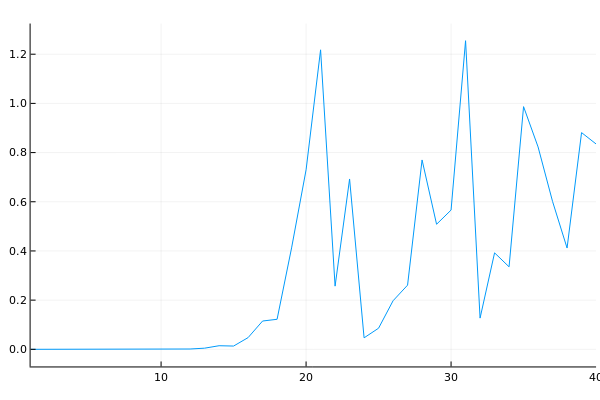
\includegraphics[width=0.49\textwidth]{zad5(1)}}\hfill
\subfloat[\texttt{Float32} i \texttt{Float64} \label{fig:zad5-2}] {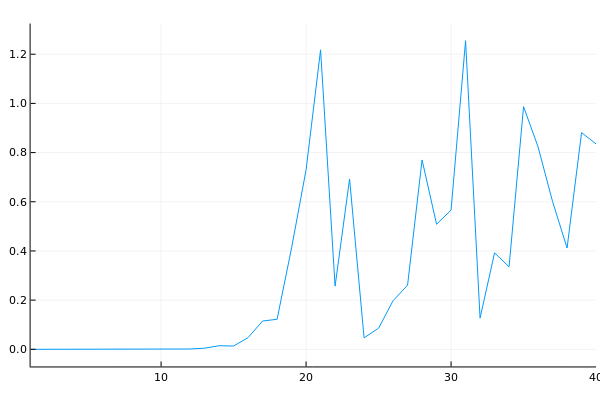
\includegraphics[width=0.49\textwidth]{zad5(2)}}\hfill
\caption{Wykresy przedstawiają różnicę pomiędzy kolejnymi wynikami iteracji} \label{fig:zad5}
\end{figure}

\subsection{Wnioski}

Przeprowadzone w zadaniu eksperymenty są przykładami sprzężenia zwrotnego, czyli procesu, w którym dane wyjściowe jednego problemu są wejściem kolejnych obliczeń. Można zatem podejrzewać, że jeżeli w pierwszym eksperymencie wynik w dziesiątej iteracji jest zgodny tylko do trzeciego miejsca po przecinku, to w dalszych iteracjach też będzie istniała różnica między wynikami. Dziwić może jednak, że wyniki wyższych iteracji wydają się zupełnie nieskorelowane. Wskazuje to na istnienie pewnego chaosu w systemie, czy też, mówiąc inaczej niemożności przewidywania (sformułowanie Lorenza). Można jednak powiedzieć, że w pierwszym eksperymencie wprowadzony błąd był zbyt duży i postawić tezę, że jeżeli błąd ten zostanie zmniejszony, to dziwne zachowanie iteracji zniknie. W tym celu przeprowadzono drugi eksperyment. Dane nie zostały w żaden sposób zaburzone, jednak do wykonywania obliczeń zostały zastosowane różne precyzje. Również tutaj widać jednak, że małe odchylenie pojawiające się w pewnym momencie jest w dalszym etapie potęgowane i znów powoduje to nieskorelowanie wyników dla późniejszych iteracji. Mogłoby się wydawać że bardziej wiarygodne są obliczenia wykonane w arytmetyce \texttt{Float64}, jednak nie jest to do końca prawdziwy wniosek, gdyż jej precyzja jest ograniczona. Można zauważyć, że w każdej kolejnej iteracji rośnie liczba cyfr znaczących pozwalających na dokładne zapisanie wyniku. W pewnym momencie zatem precyzja arytmetyki \texttt{Float64} staje się niewystarczająca. Widać zatem, że niezależnie od tego, jak małe odchylenie od wartości początkowych zostanie wybrane, na skutek przeniesienia błędu jako wejście do kolejnej iteracji, a potem następnej, itd., będzie on gwałtownie rósł, tak że po stosunkowo niewielu iteracjach przewidywanie za pomocą komputera stanie się bezwartościowe. Zaobserwowana tutaj numeryczna niestabilność jest ciężka do uniknięcia, ponieważ nie istnieje arytmetyka o nieskończonej precyzji, która byłaby w stanie wykonać wszystkie obliczenia poprawnie, można jedynie przez wybór odpowiednio dużej precyzji opóźnić zjawisko niemożności przewidywania.

\section{Iterowanie funkcji kwadratowej}

\subsection{Opis problemu}

Zbadanie zachowania równania rekurencyjnego
\begin{align}
x_{n+1} := x^2_n + c, \ \textrm{dla} \ n = 0,1,\dots,
\label{eq:zad6}
\end{align}
gdzie $c$ jest pewną daną stałą, dla następujących danych:
\begin{enumerate}[(i)]
\item $c = -2$ i $x_0 = 1$
\item $c = -2$ i $x_0 = 2$
\item $c = -2$ i $x_0 = 1.99999999999999$
\item $c = -1$ i $x_0 = 1$
\item $c = -1$ i $x_0 = -1$
\item $c = -1$ i $x_0 = 0.75$
\item $c = -1$ i $x_0 = 0.25$
\end{enumerate}
W tym celu należało wykonać 40 iteracji wyrażenia \eqref{eq:zad6} i zaobserwować zachowanie generowanych ciągów, a także przeprowadzić iterację graficzną \eqref{eq:zad6}. 

\subsection{Rozwiązanie}

Zaimplementowano wyrażenie \eqref{eq:zad6} i za pomocą stworzonej w programie funkcji dla danych parametrów wejściowych $x_0$ i $c$ wykonano zadaną liczbę iteracji.

\subsection{Wyniki}

Wyniki kolejnych iteracji wyrażenia \eqref{eq:zad6} dla różnych danych wejściowych przedstawia \Cref{table:8}.

\begin{table}[h]
        \centering
        \scriptsize
\begin{tabular}{c
		|S[
        table-number-alignment = right,
		table-figures-integer  = 2,
		table-figures-decimal = 1,
		%table-figures-exponent=6
		]
		|S[
        table-number-alignment = right,
		table-figures-integer  = 2,
		table-figures-decimal = 1,
		%table-figures-exponent=6
		]
		|S[
        table-number-alignment = right,
		table-figures-integer  = 2,
		table-figures-decimal = 16,
		%table-figures-exponent=6
		]
		|S[
        table-number-alignment = right,
		table-figures-integer  = 2,
		table-figures-decimal = 1,
		%table-figures-exponent=6
		]
		|S[
        table-number-alignment = right,
		table-figures-integer  = 2,
		table-figures-decimal = 1,
		%table-figures-exponent=6
		]
		|S[
        table-number-alignment = right,
		table-figures-integer  = 2,
		table-figures-decimal = 16,
		table-figures-exponent=2
		]
		|S[
        table-number-alignment = right,
		table-figures-integer  = 2,
		table-figures-decimal = 15,
		table-figures-exponent=2
		]}
%\toprule
\multirow{2}{*}{It.} & \multicolumn{3}{c|}{$c=-2$} & \multicolumn{4}{c}{$c=-1$}  \\ \cline{2-8}
&{$x_0$=1}&{$x_0$=2}&{$x_0$=1.99999999999999}&{$x_0$=1}&{$x_0$=-1}&{$x_0$=0.75}&{$x_0$=0.25} \\ \hline
1&-1.0&2.0&1.99999999999996&0.0&0.0&-0.4375&-0.9375 \\
2&-1.0&2.0&1.9999999999998401&-1.0&-1.0&-0.80859375&-0.12109375 \\
3&-1.0&2.0&1.9999999999993605&0.0&0.0&-0.3461761474609375&-0.9853363037109375 \\
4&-1.0&2.0&1.999999999997442&-1.0&-1.0&-0.8801620749291033&-0.029112368589267135 \\
5&-1.0&2.0&1.9999999999897682&0.0&0.0&-0.2253147218564956&-0.9991524699951226 \\
6&-1.0&2.0&1.9999999999590727&-1.0&-1.0&-0.9492332761147301&-0.0016943417026455965 \\
7&-1.0&2.0&1.999999999836291&0.0&0.0&-0.0989561875164966&-0.9999971292061947 \\
8&-1.0&2.0&1.9999999993451638&-1.0&-1.0&-0.9902076729521999&-5.741579369278327e-6 \\
9&-1.0&2.0&1.9999999973806553&0.0&0.0&-0.01948876442658909&-0.9999999999670343 \\
10&-1.0&2.0&1.999999989522621&-1.0&-1.0&-0.999620188061125&-6.593148249578462e-11 \\
11&-1.0&2.0&1.9999999580904841&0.0&0.0&-0.0007594796206411569&-1.0 \\
12&-1.0&2.0&1.9999998323619383&-1.0&-1.0&-0.9999994231907058&0.0 \\
13&-1.0&2.0&1.9999993294477814&0.0&0.0&-1.1536182557003727e-6&-1.0 \\
14&-1.0&2.0&1.9999973177915749&-1.0&-1.0&-0.9999999999986692&0.0 \\
15&-1.0&2.0&1.9999892711734937&0.0&0.0&-2.6616486792363503e-12&-1.0 \\
16&-1.0&2.0&1.9999570848090826&-1.0&-1.0&-1.0&0.0 \\
17&-1.0&2.0&1.999828341078044&0.0&0.0&0.0&-1.0 \\
18&-1.0&2.0&1.9993133937789613&-1.0&-1.0&-1.0&0.0 \\
19&-1.0&2.0&1.9972540465439481&0.0&0.0&0.0&-1.0 \\
20&-1.0&2.0&1.9890237264361752&-1.0&-1.0&-1.0&0.0 \\
21&-1.0&2.0&1.9562153843260486&0.0&0.0&0.0&-1.0 \\
22&-1.0&2.0&1.82677862987391&-1.0&-1.0&-1.0&0.0 \\
23&-1.0&2.0&1.3371201625639997&0.0&0.0&0.0&-1.0 \\
24&-1.0&2.0&-0.21210967086482313&-1.0&-1.0&-1.0&0.0 \\
25&-1.0&2.0&-1.9550094875256163&0.0&0.0&0.0&-1.0 \\
26&-1.0&2.0&1.822062096315173&-1.0&-1.0&-1.0&0.0 \\
27&-1.0&2.0&1.319910282828443&0.0&0.0&0.0&-1.0 \\
28&-1.0&2.0&-0.2578368452837396&-1.0&-1.0&-1.0&0.0 \\
29&-1.0&2.0&-1.9335201612141288&0.0&0.0&0.0&-1.0 \\
30&-1.0&2.0&1.7385002138215109&-1.0&-1.0&-1.0&0.0 \\
31&-1.0&2.0&1.0223829934574389&0.0&0.0&0.0&-1.0 \\
32&-1.0&2.0&-0.9547330146890065&-1.0&-1.0&-1.0&0.0 \\
33&-1.0&2.0&-1.0884848706628412&0.0&0.0&0.0&-1.0 \\
34&-1.0&2.0&-0.8152006863380978&-1.0&-1.0&-1.0&0.0 \\
35&-1.0&2.0&-1.3354478409938944&0.0&0.0&0.0&-1.0 \\
36&-1.0&2.0&-0.21657906398474625&-1.0&-1.0&-1.0&0.0 \\
37&-1.0&2.0&-1.953093509043491&0.0&0.0&0.0&-1.0 \\
38&-1.0&2.0&1.8145742550678174&-1.0&-1.0&-1.0&0.0 \\
39&-1.0&2.0&1.2926797271549244&0.0&0.0&0.0&-1.0 \\
40&-1.0&2.0&-0.3289791230026702&-1.0&-1.0&-1.0&0.0 \\
%\bottomrule
\end{tabular}
\caption{Kolejne iteracje funkcji $x_{n+1}=x_n^2 + c$ dla danych $x_0$ i $c$}
\label{table:8}
\end{table}

\noindent W celu lepszego przedstawienia wyników metodą iteracji graficznej zostały stworzone wykresy, które przedstawia \Cref{fig:zad6}.

\begin{figure}[h]
\centering
\subfloat[$x_{n+1}=x_n^2 - 2$\label{fig:zad6-1}]{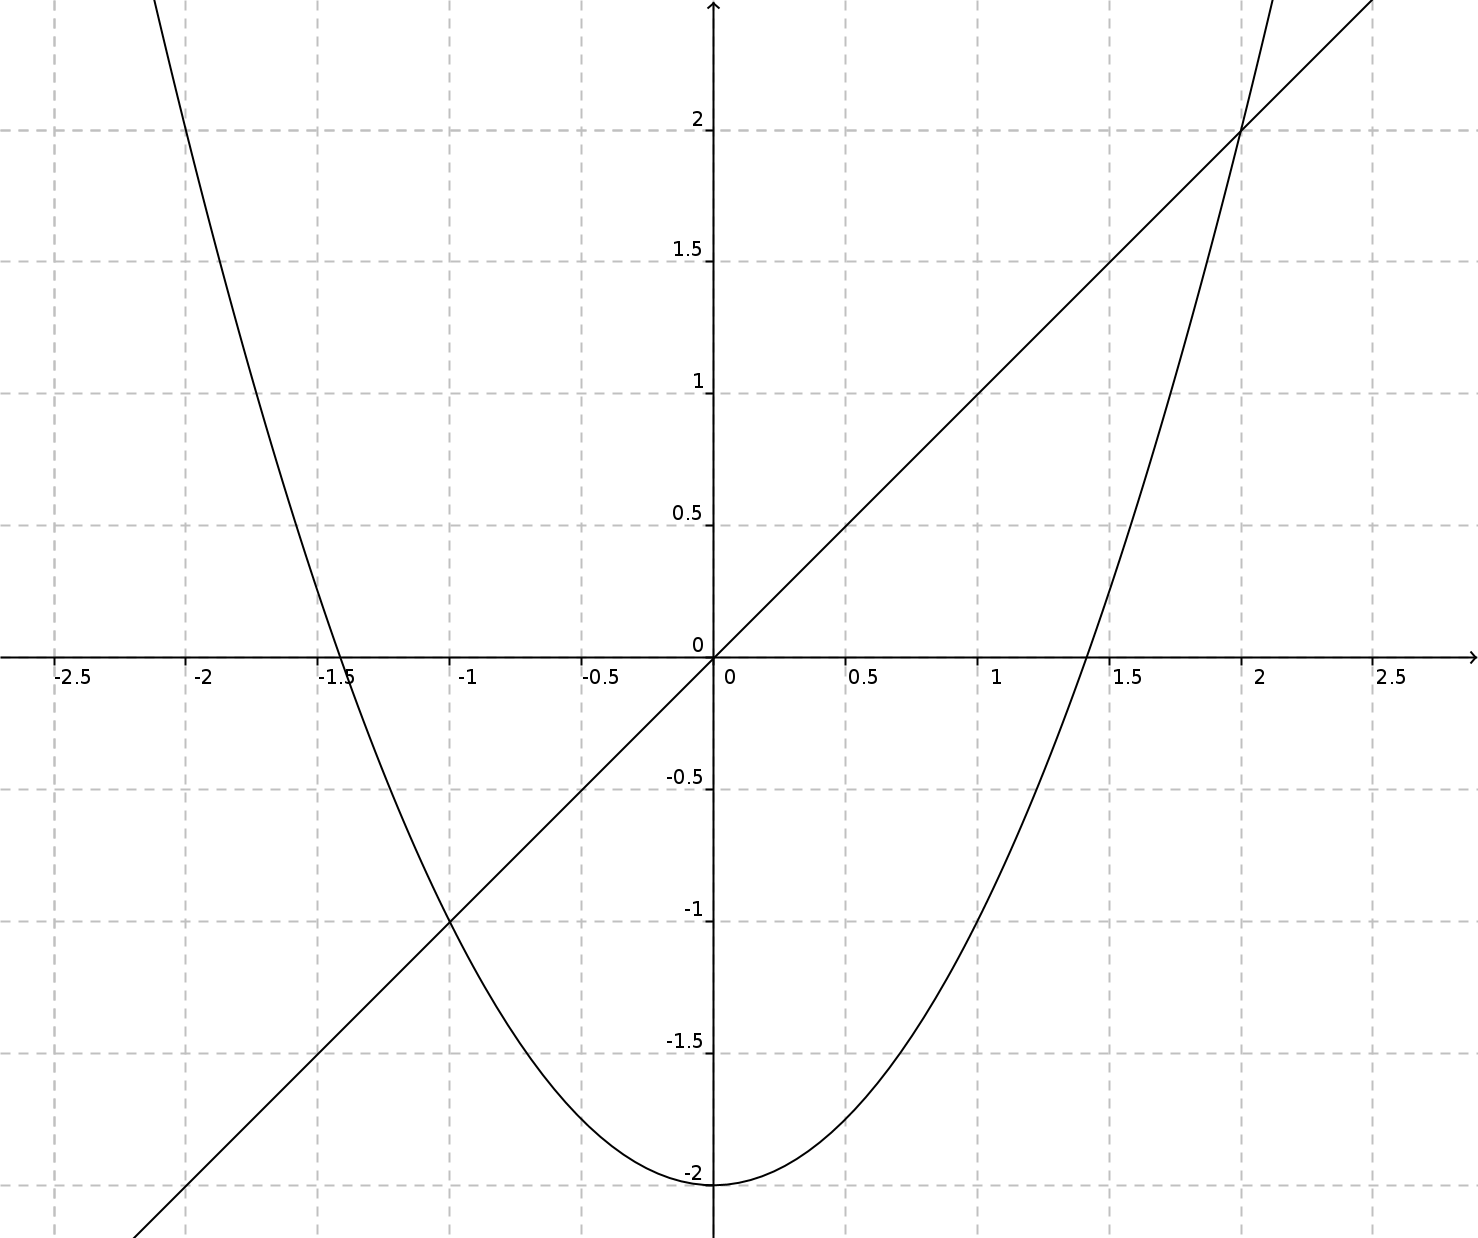
\includegraphics[width=0.5\textwidth]{zad61}}\hfill
\subfloat[$x_{n+1}=x_n^2 - 1$\label{fig:zad6-6}] {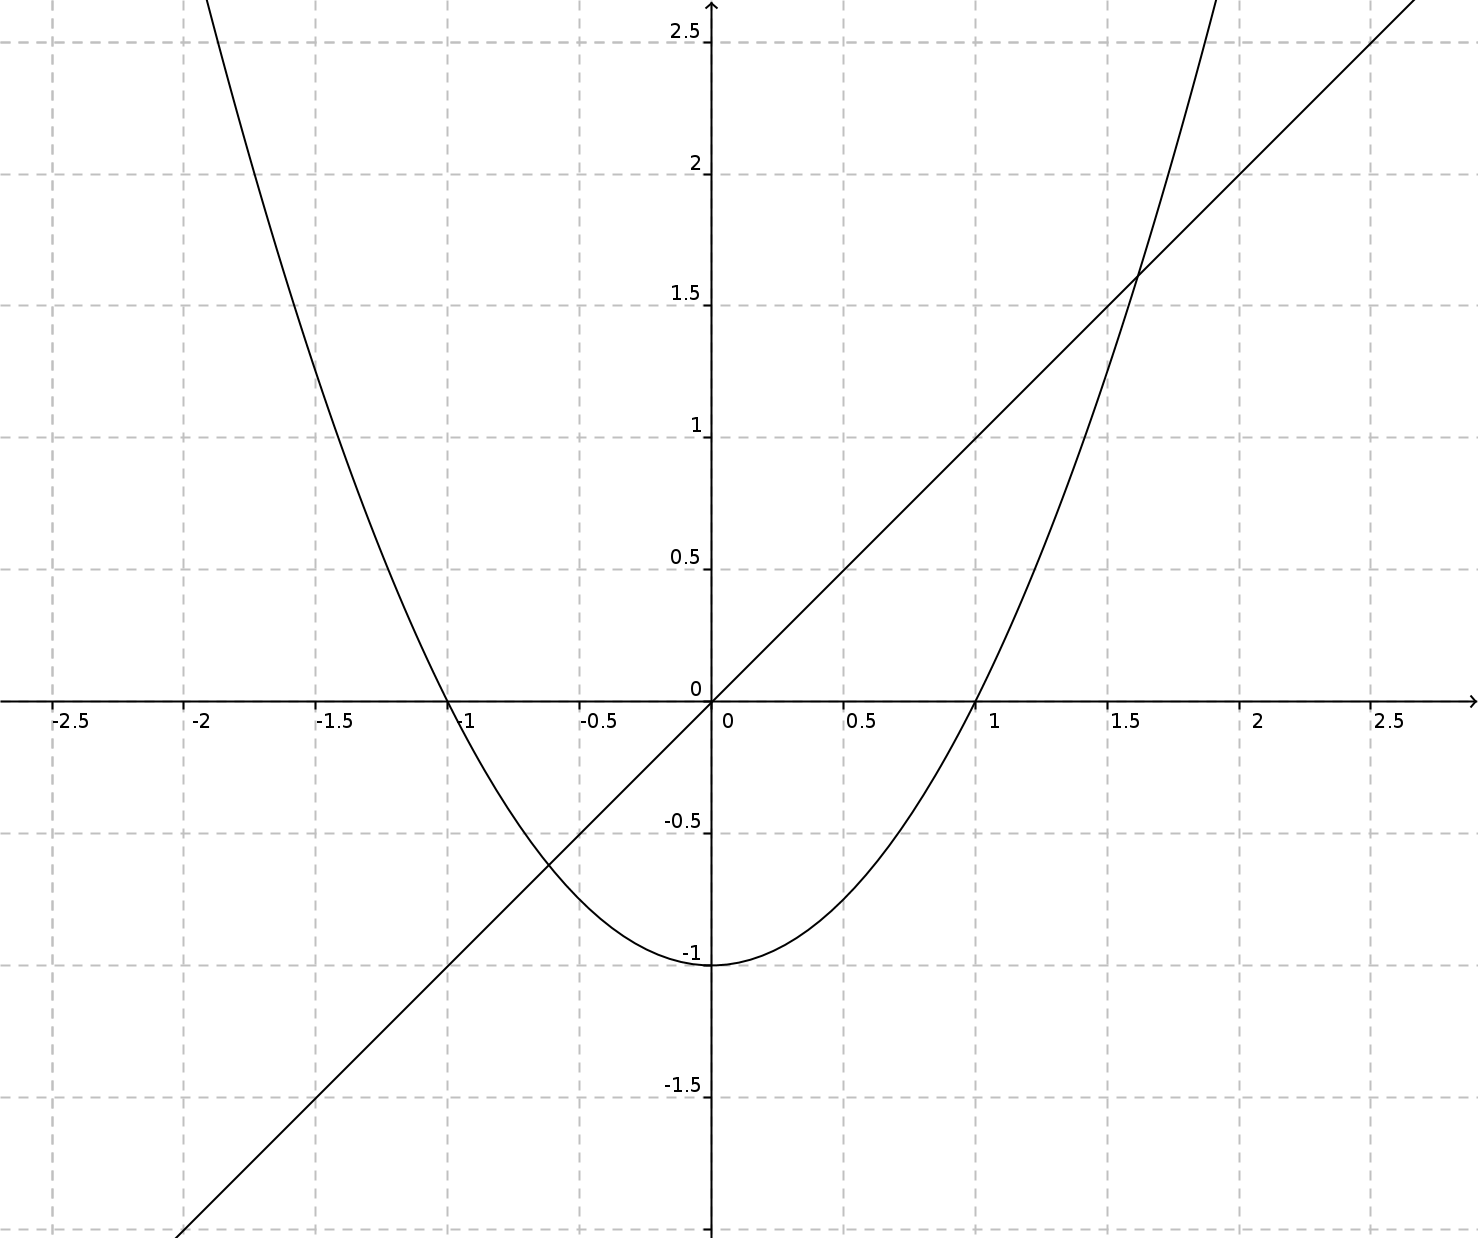
\includegraphics[width=0.5\textwidth]{zad62}}\hfill
\subfloat[$x_0 = 1, c = -2$\label{fig:zad6-11}]{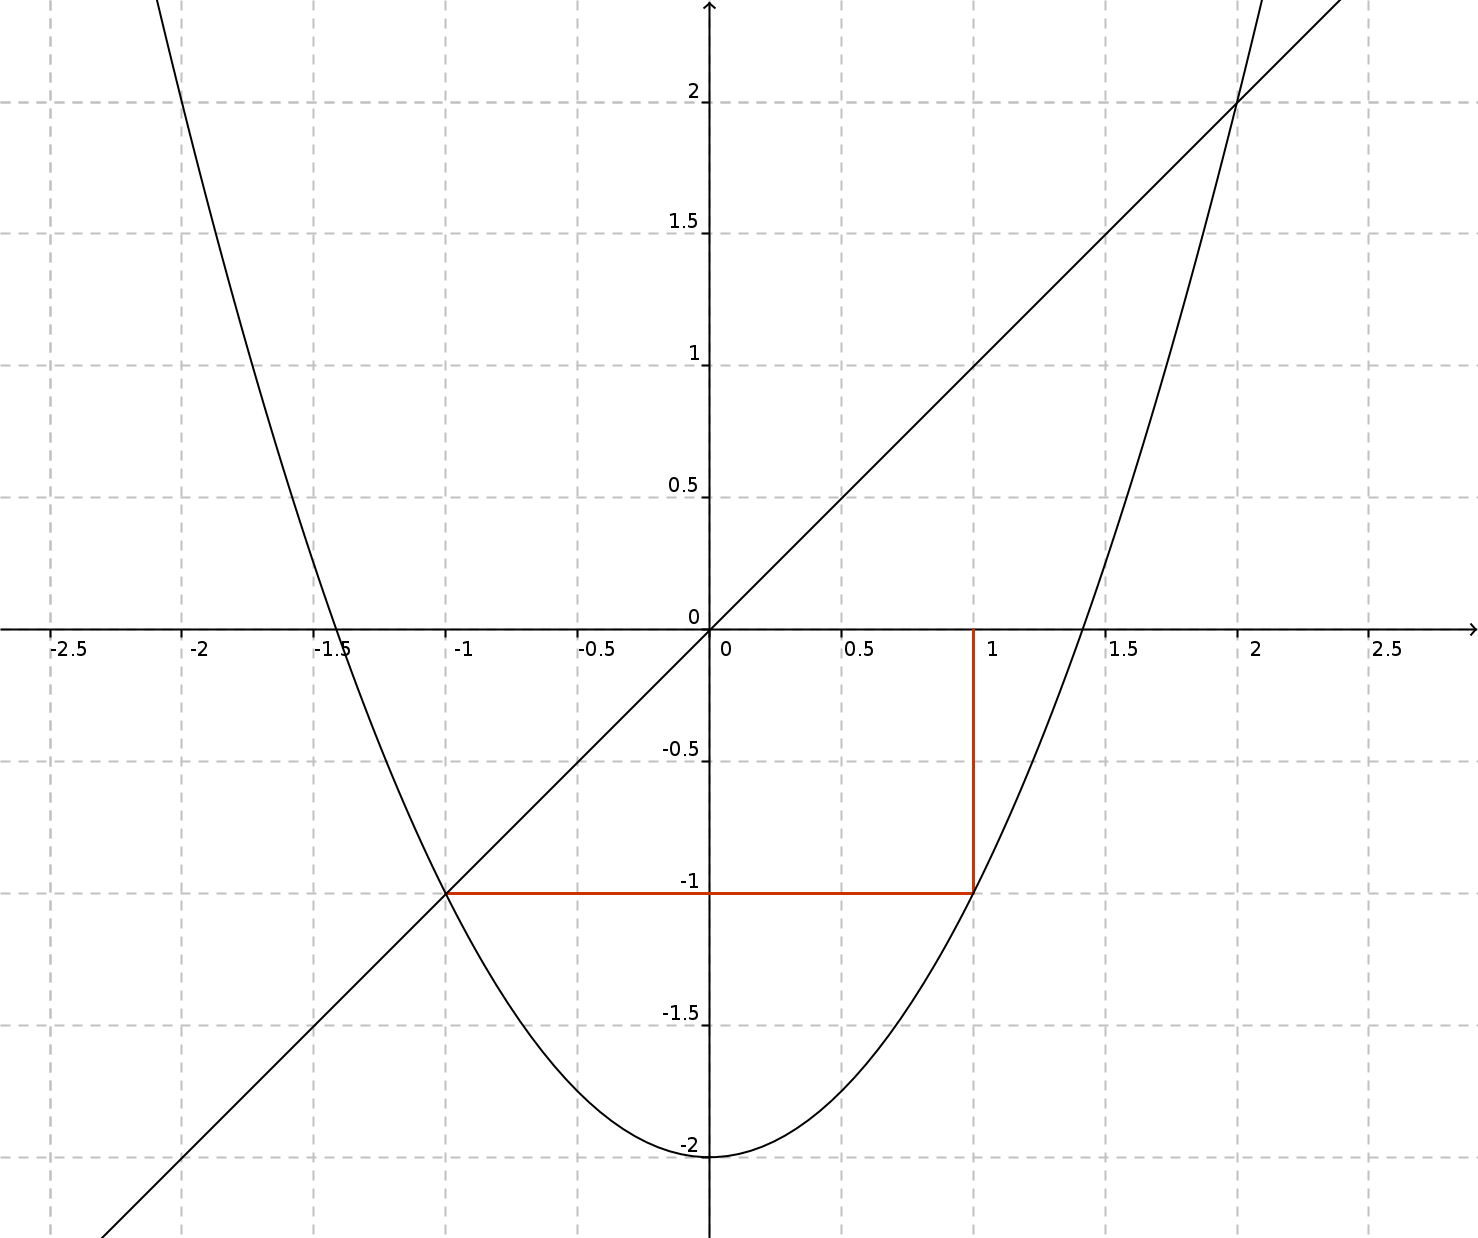
\includegraphics[width=0.5\textwidth]{zad611}}\hfill
\subfloat[$x_0 = 1, c = -1$\label{fig:zad6-21}]{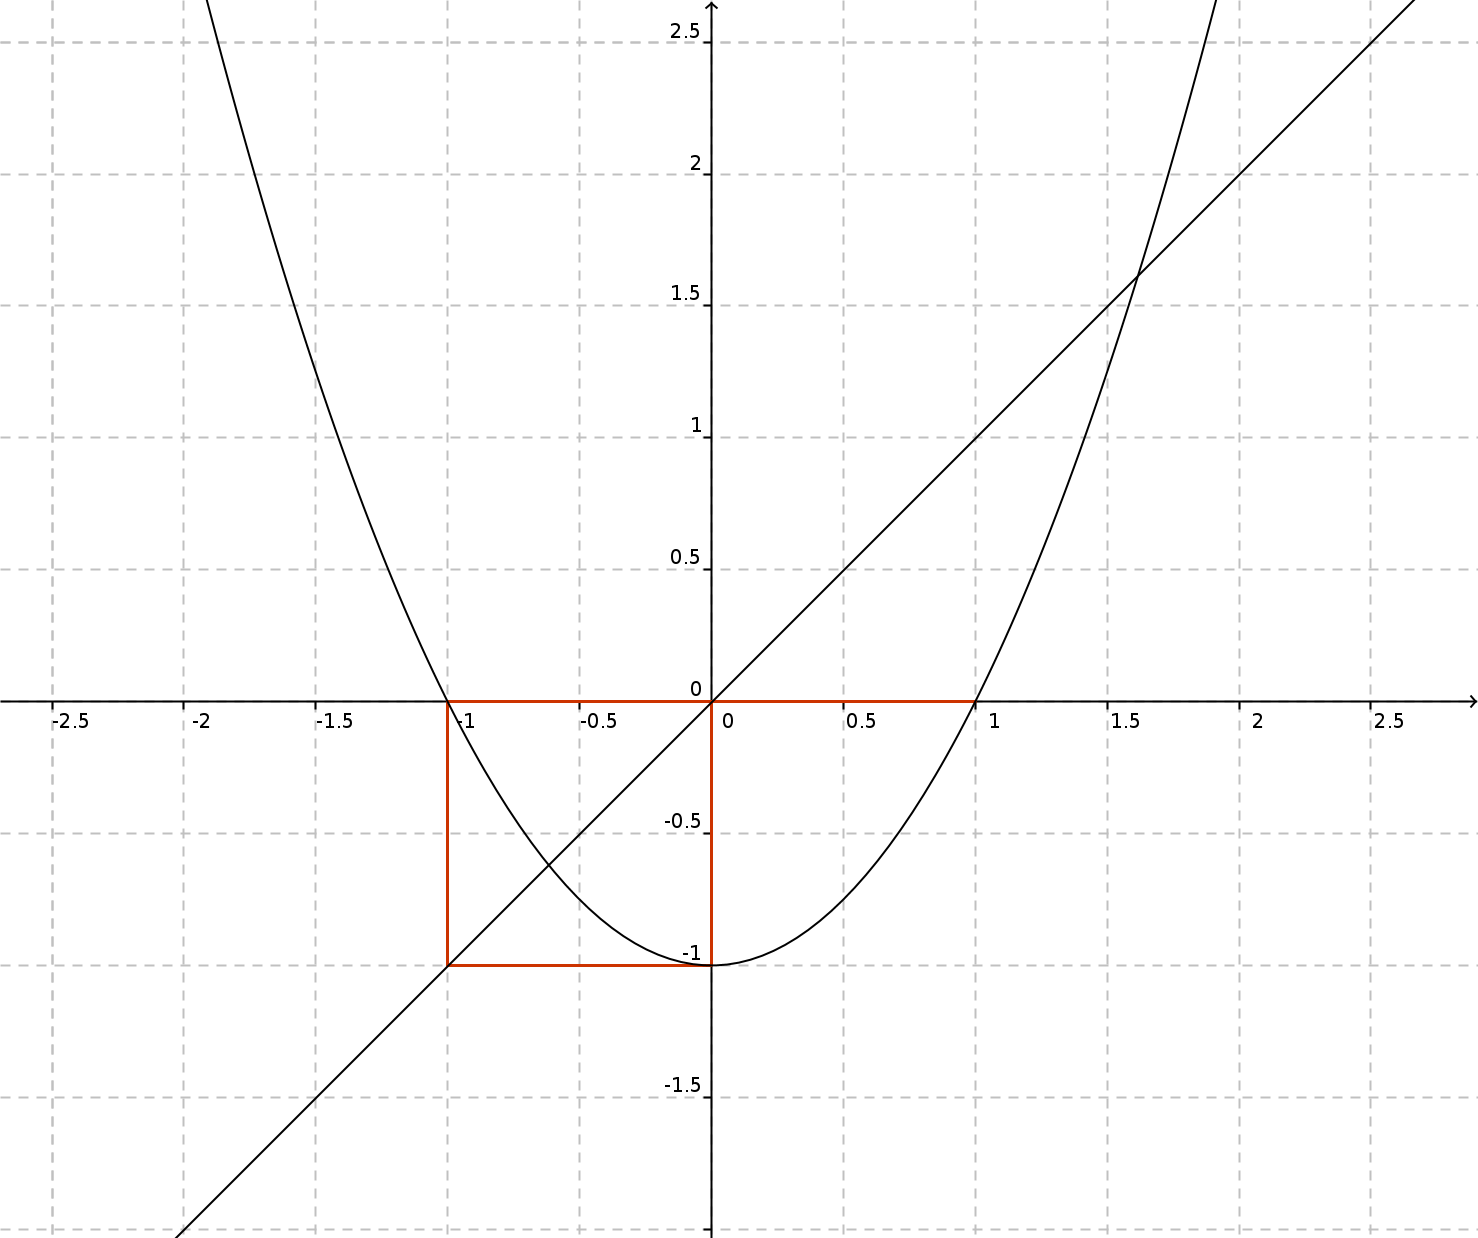
\includegraphics[width=0.5\textwidth]{zad621}}\hfill
\caption{Iteracje graficzne wyrażenia $x_{n+1}=x_n^2 + c$ dla wybranych $x_0$ i $c$}
\label{fig:zad6}
\end{figure}
\begin{figure}[h]\ContinuedFloat
\centering
\subfloat[$x_0 = 0.25, c = -1$\label{fig:zad6-225}]{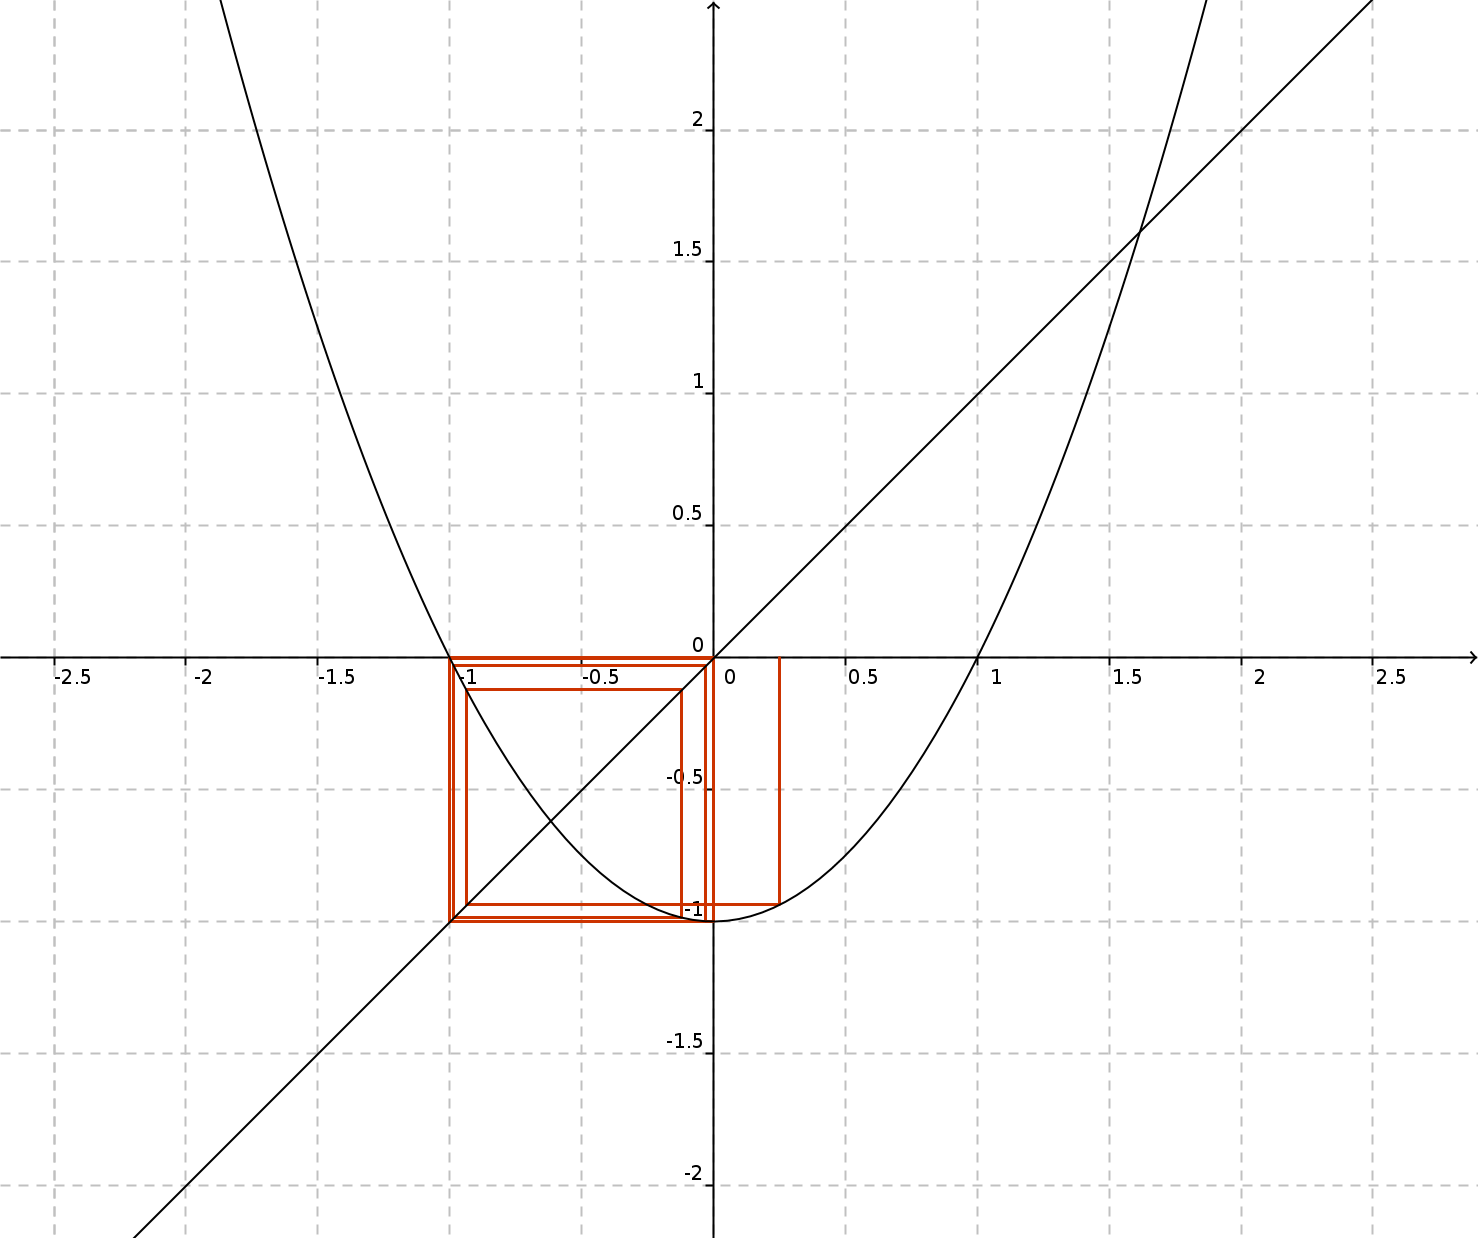
\includegraphics[width=0.5\textwidth]{zad6225}}\hfill
\subfloat[$x_0 = 0.75, c = -1$\label{fig:zad6-275}]{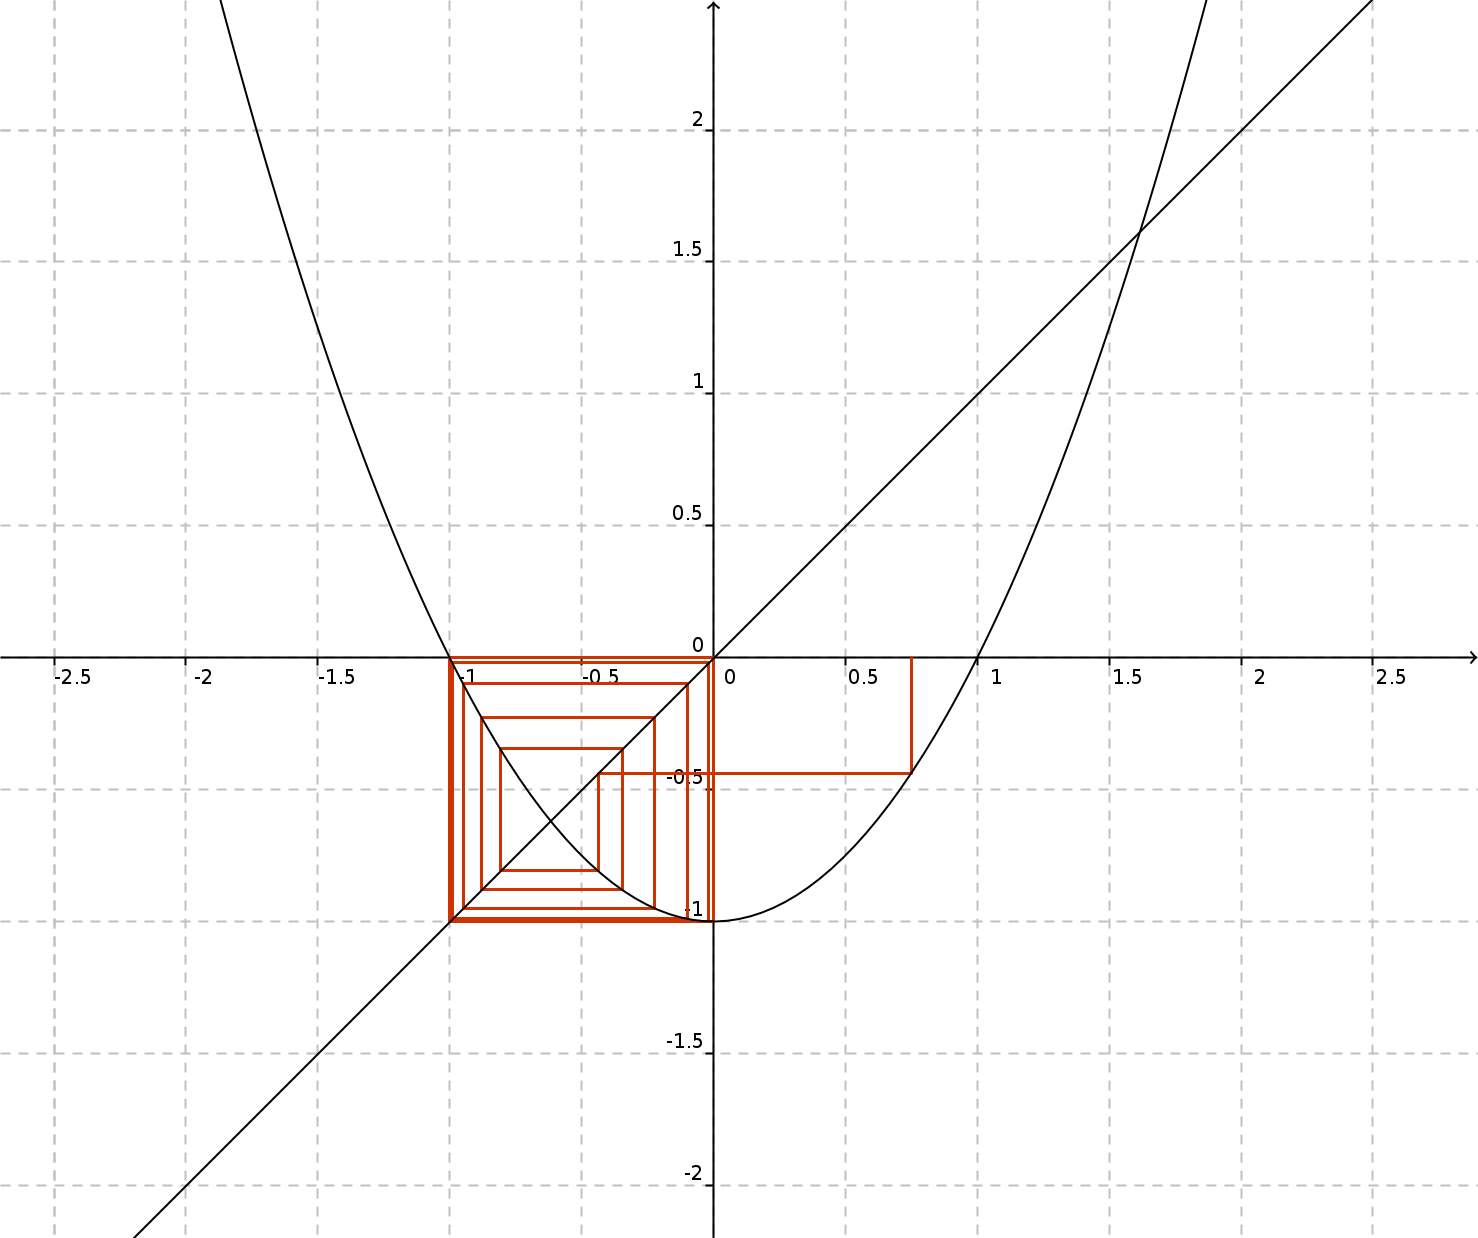
\includegraphics[width=0.5\textwidth]{zad6275}}\hfill
\subfloat[$x_0 = 1.99999999999999, c = -2$ -- 40 iteracji\label{fig:zad6-191}]{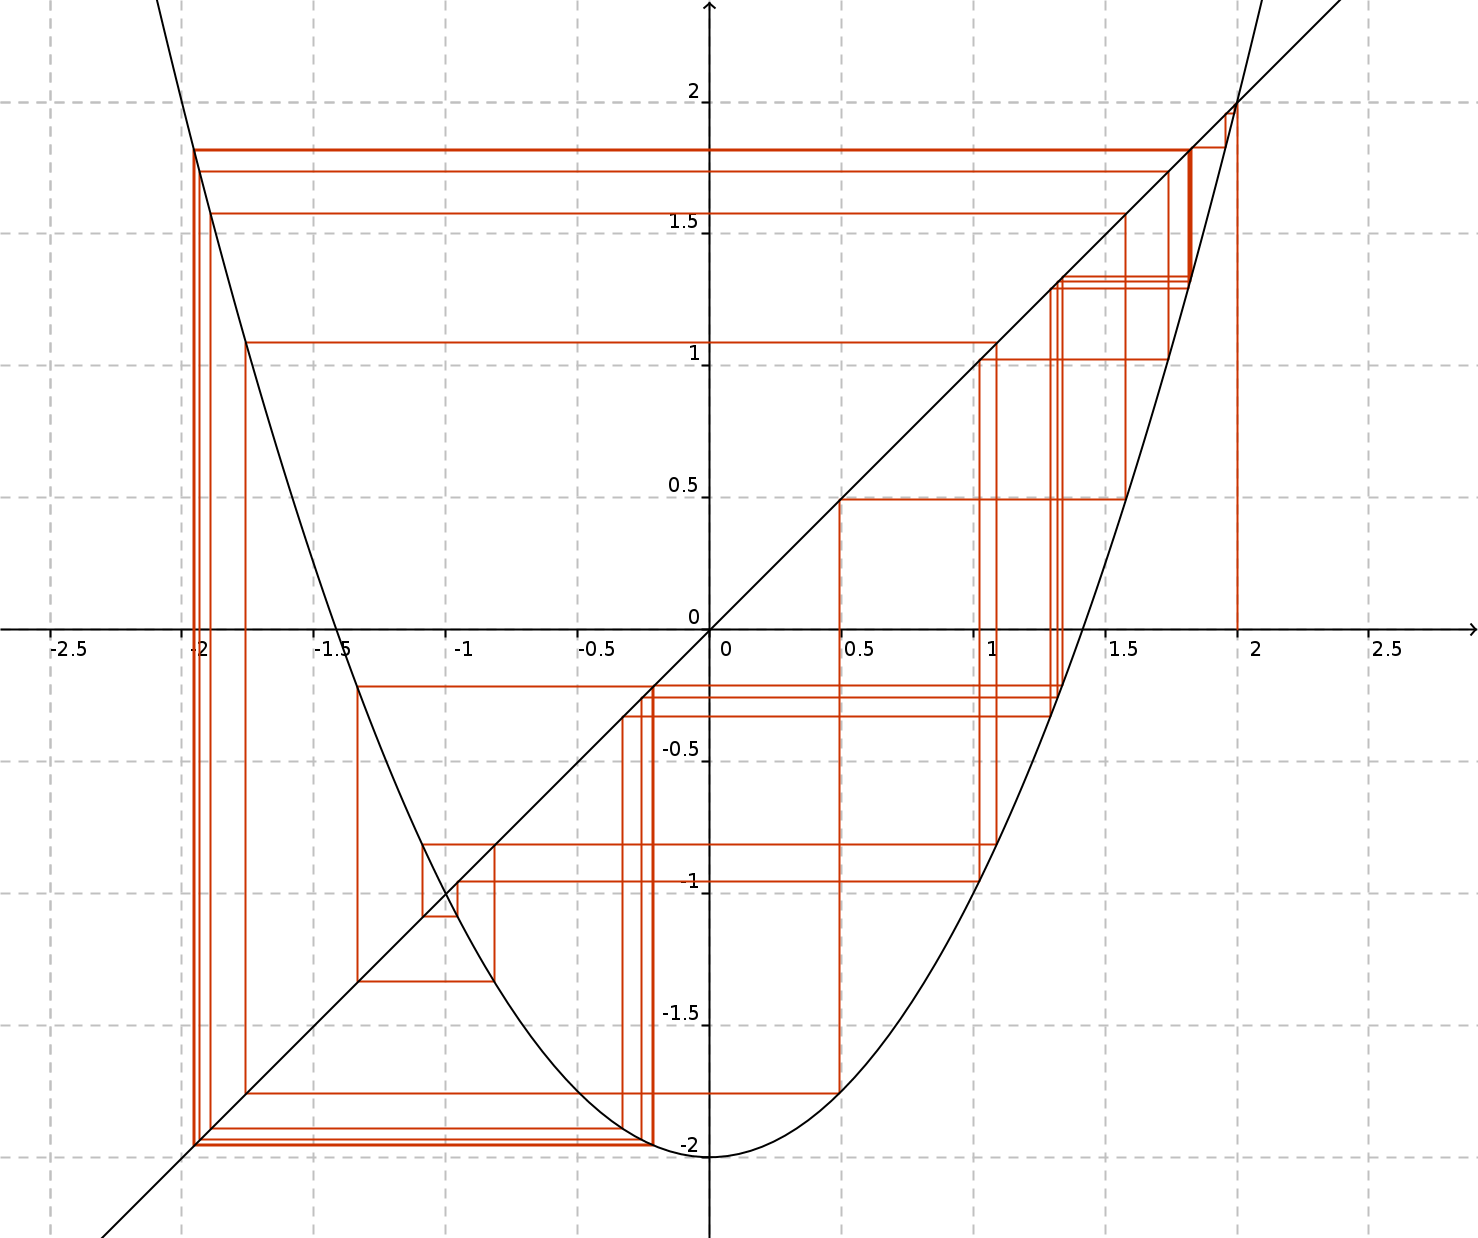
\includegraphics[width=0.5\textwidth]{zad6191}}\hfill
\subfloat[$x_0 = 1.99999999999999, c = -2$ -- 100 iteracji\label{fig:zad6-192}]{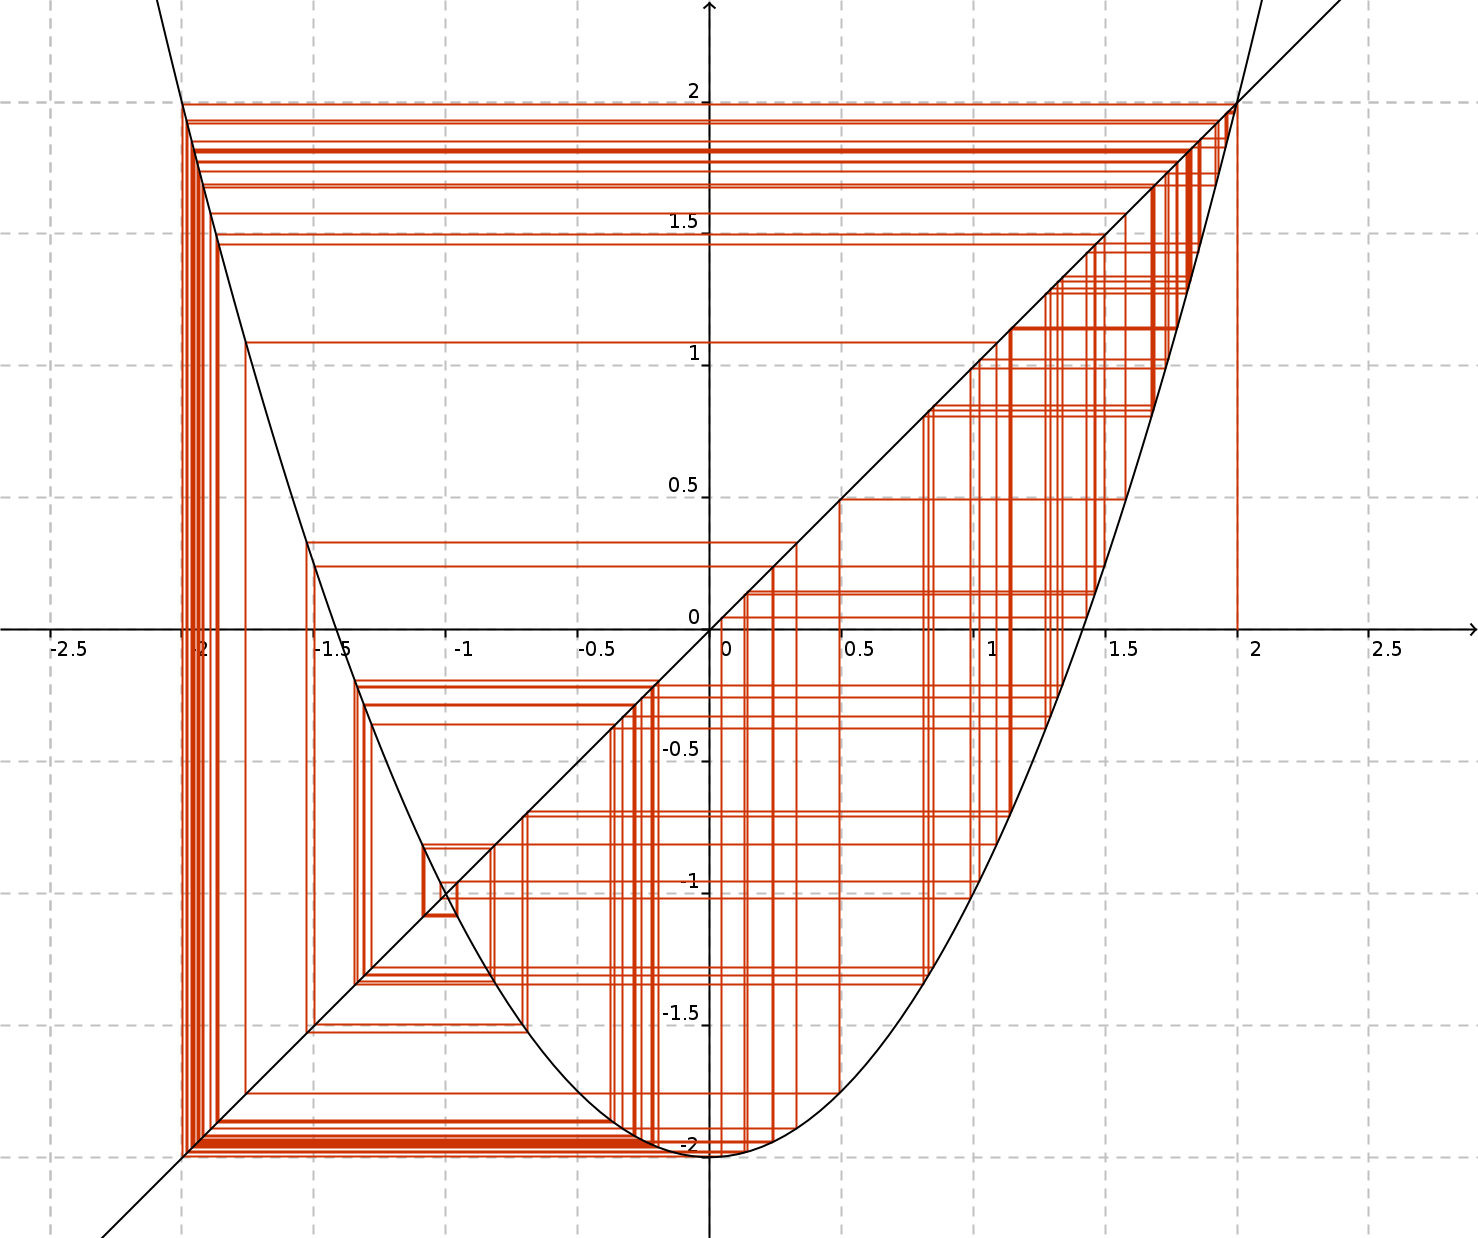
\includegraphics[width=0.5\textwidth]{zad6192}}\hfill
\subfloat[$x_0 = 1.99999999999999, c = -2$ -- 200 iteracji\label{fig:zad6-193}]{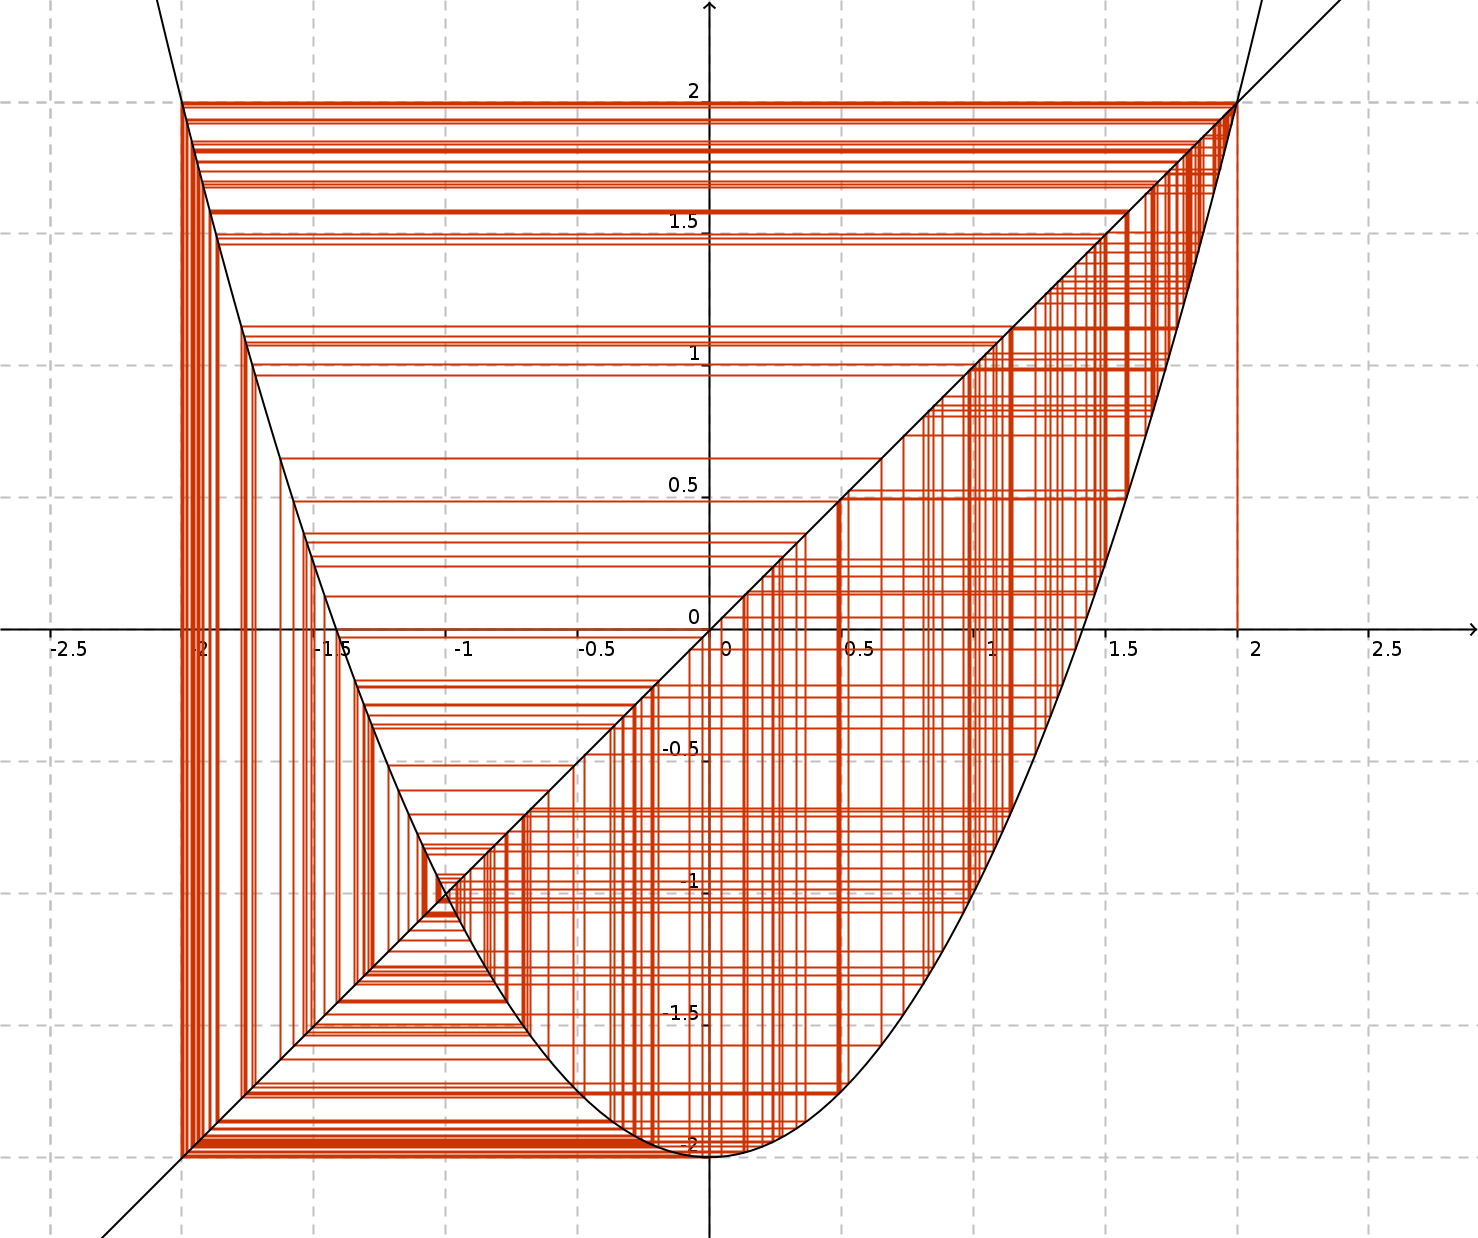
\includegraphics[width=0.5\textwidth]{zad6193}}\hfill
\caption{Iteracje graficzne wyrażenia $x_{n+1}=x_n^2 + c$ dla wybranych $x_0$ i $c$} 
\end{figure}

\subsection{Wnioski}

Analizując zadanie poprzednie (model wzrostu populacji) można wyciągnąć wnioski, że za niestabilność numeryczną odpowiedzialna jest tylko i wyłącznie operacja podnoszenia do kwadratu. Iteracje wykonane w tym zadaniu obalają jednak ten wniosek. W tabeli \ref{table:8} widać, że dla $x_0 = 1$ lub $x_0 = 2$ przy $c = -2$ iteracja zachowuje się stabilnie. W przypadku, gdy $x_0 = 1.99999999999999$ (jest to niewielkie odchylenie od $2$) widać natomiast odmienne zachowanie, w którym występuje niestabilność. Doskonale obrazuje to metoda iteracji graficznej pokazana na wykresach \ref{fig:zad6-191}, \ref{fig:zad6-192}, \ref{fig:zad6-193}. Można zatem wyciągnąć wnioski, że niektóre z danych początkowych prowadzą do stabilnego zachowania, inne generują niestabilność wyników. W rzeczywistości w przedziale $[-2, 2]$ nie znajduje się zbyt wiele wartości prowadzących do rozwiązań stabilnych. Funkcja $\phi(x) = x^2 - 2$ posiada dwa punkty stałe (tzn. takie $x$ dla których $\phi(x) = x$) -- $-1$, $2$, co pokazuje wykres \ref{fig:zad6-1}. Wartości początkowe dla których $\phi(x)$ jest zbieżna do tych punktów prowadzą do stabilnych rozwiązań. Eksperymentalne sprawdzenie za pomocą iteracji graficznej pokazało jednak że w dużej mierze $\phi(x)$ jest rozbieżna. Zbieżność została zaobserwowana dla pojedynczych wartości $x_0$ takich jak: $-2, -1, 0, 1, 2$. Obserwacje te pokazują, że analiza błędu nie jest łatwa do przeprowadzenia, co staje się jeszcze bardziej widoczne kiedy wartość $c = -2$ została zamieniona na $c = -1$. Dla tak zdefiniowanej funkcji $\phi(x)$ otrzymano punkty stałe $\dfrac{1-\sqrt{5}}{2}$ i $\dfrac{1+\sqrt{5}}{2}$. Zaobserwować można jednak inną ciekawą rzecz. Startując od $x_0$ równego $1, -1, 0.75$ czy $0.25$ po pewnej liczbie iteracji proces ustala się i powtarzają się tylko dwie wartości: $0$ i $-1$. Do takiego efektu doprowadza również wybranie wielu innych wartości początkowych. Dla takich wartości $x_0$ układ sprzężenia zwrotnego jest w stanie idealnie stabilnym, co obrazują wykresy \ref{fig:zad6-21}, \ref{fig:zad6-275} i \ref{fig:zad6-225}. Dla tak przewidywalnych procesów niewielkie błędy podczas przebiegu zanikają lub ulegają redukcji, mogą więc zostać pominięte. Można posłużyć się zatem arytmetyką o skończonej precyzji, która staje się narzędziem jak najbardziej zdatnym do analizy i nie może zawieść.

%\begin{algorithm}[h]
%\caption{Wyznaczanie epsilonów maszynowych.}
%\label{alg:macheps}
%\SetKwData{Macheps}{macheps}\SetKwData{NMacheps}{new\_{}macheps}
%
%\Macheps $\leftarrow 1.0$\;
%\NMacheps $\leftarrow 1.0$\;
%\While {$1.0 + \NMacheps > 1.0$}{
%$\Macheps\leftarrow \NMacheps$\;
%$\NMacheps \leftarrow \NMacheps / 2.0$\;
%}
%\Return \Macheps
%\end{algorithm}

\end{document}
